\documentclass{report}
\usepackage{amsmath}
\usepackage{amssymb}
\usepackage[hmargin=2.5cm,vmargin=2.5cm]{geometry}
\usepackage{tabularx}
\usepackage{booktabs}
%\usepackage{biblatex}
%\bibliography{thesis.bib}
\usepackage{graphicx}
\usepackage{color}
\usepackage{wrapfig}
\usepackage{multirow}
\usepackage{multicol}
%\usepackage{cite}
\usepackage[rightcaption]{sidecap}
%\usepackage{hyperref}
\usepackage{threeparttable}
\usepackage[table]{xcolor}
\usepackage{psfrag}
\usepackage[margin=10pt,font=small,textfont=sf,labelfont=bf]{caption}
\usepackage{subfig}
\usepackage[section]{placeins}

\begin{document}
\bibliographystyle{plain}

\chapter{1}

\chapter{Tower Support Structure Design}

\section{Abstract}
This study examines two possible alterations to the detector towers for the SuperCDMS Experiment.
The first modification involves alternate support tube materials to act as thermal isolators for
separate tower stages. Candidates are chosen for low thermal conductivity, low radioactivity,
and high strength. The thermal conductivity of Vespel SCP-5000, Vespel SCP-5050, Ti 15-3-3-3,
and Ti21S are measured. The gamma radioactivity of all samples were measured. The radius and
thickness of the tubes were then optimized to minimize radioactivity and thermal power loading
to each stage. The second design alteration proposes low inductance parallel-strip transmission
lines to replace current vacuum coaxial wires on the tower face. The thermal loads and inductance
calculations are presented.

\begin{raggedleft}
\setlength{\unitlength}{2cm}
\begin{picture}(5,0)
\thicklines
\put(0,0){\line(1,0){7}}
\end{picture}
\end{raggedleft}

\begin{multicols}{2}

\section{Introduction}
The CDMS (Cryogenic Dark Matter Search) Experiments

\begin{itemize}
\item search for dark matter CDMS in general
\item detector operation, limited cooling power, limiting thermal conductivity, limiting
radioactivity.
\end{itemize}
\section{Tower Support Tube Design}
We are proposing design alterations for SNOLab, considering possible alternate materials
and dimensions for the central support tubes.

\bigskip

Considerations for Material Candidates:
\begin{itemize}
\item Thermal Conductivity
\item Radioactivity
\item Mechanical Properties
\end{itemize}

\subsection{Thermal Conductivity}
Due to the finite cooling power of our helium dilution refrigerator, we must limit the
thermal load to each stage of the fridge. The tower support tubes are a major source of
thermal loading on each stage. The thermal power load on each stage from the tubes is
governed by the general equation
\begin{eqnarray}
Power = \int_{T_{low}}^{T_{high}} \frac{A}{L}K(T)dT \ \ , %place this above in a more general section and reference it.
\end{eqnarray}
where $T_{low}$ is the temperature of the stage being loaded, $T_{high}$ is the warmer
connecting stage, A is the tube cross-sectional area, L is tube length, and K(T) is the
thermal conductivity. From the equation, we can see that thermal power is directly proportional
to thermal conductivity, so by decreasing thermal conductivity, we decrease power to each
stage. Figure 1 displays the thermal conductivity for tower tube candidate materials.
\begin{figure}[htb]
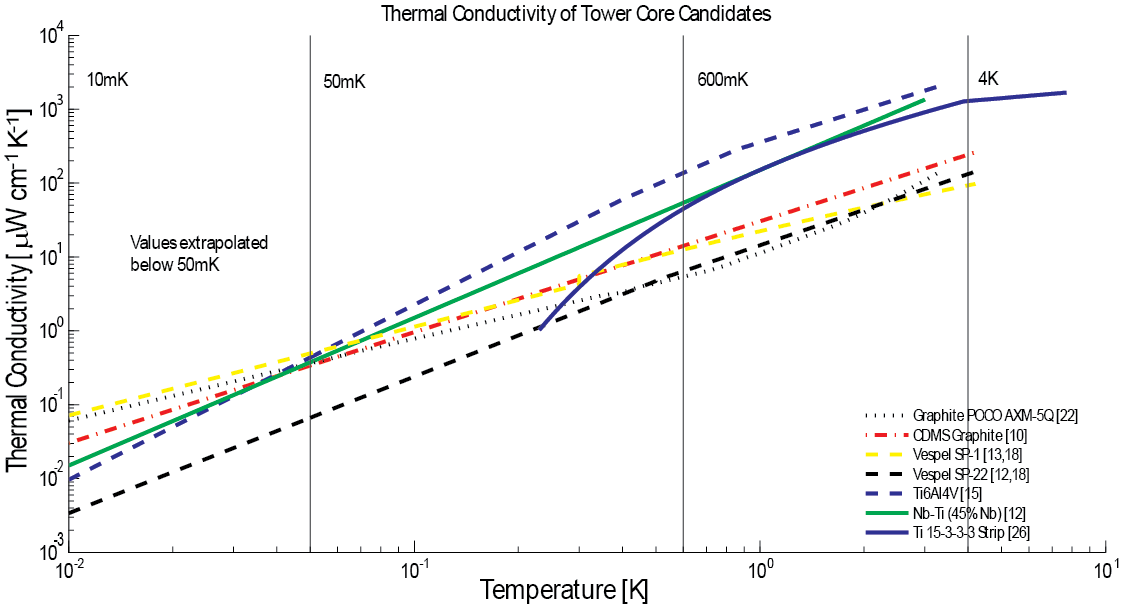
\includegraphics[width = \textwidth]{TowerCond.png}
\caption{Thermal conductivity of the various core material candidates. All values have been
extrapolated past 50mK. Below are the materials which offer improvement over UF-4S
graphite for each stage.}
\end{figure}
\begin{figure}[htb]
\centering
\begin{minipage}[t]{.3\textwidth}
\textbf{4K - 600mK Stage:}
\begin{itemize}
\item Vespel SP-1
\item Vespel SP-22
\item POCO AXM-5Q
\end{itemize}
\end{minipage}
\begin{minipage}[t]{.3\textwidth}
\textbf{600mK - 50mK Stage:}
\begin{itemize}
\item POCO AXM-5Q
\item Vespel SP-22
\item Vespel SP-1
\end{itemize}
\end{minipage}
\begin{minipage}[t]{.3\textwidth}
\textbf{50mK-10mK Stage:}
\begin{itemize}
\item Vespel SP-22
\item Ti 15-3-3-3
\end{itemize}
\end{minipage}
\end{figure}

From the graph, one can see that Ti 15-3-3-3 potentially has a much lower thermal
conductivity for the temperature range of the lowest support tube, 100mK to 40mK.
Current data only extends down to 230mK, however. At that temperature, it is crossing
the lowest thermally conductive material, Vespel SP-22, and decreasing quickly.

Table 1 summarizes the possible improvements in thermal power conducted for each stage,
assuming identical tube dimensions.

\begin{table}[htb]
\begin{threeparttable}
{\footnotesize\rm\begin{tabularx}{17.7cm}{l|XXXXXX}
  \multicolumn{7}{l}{{\large Calculated Power Conducted for Candidate Tower Materials}}\\
\toprule
 {\normalsize Material} & 4.2K-600mK  &5K-1K\tnote{*}& 600mK-50mK & 1K-100mK\tnote{*} & 50mK-10mK & 100mK-40mK\tnote{*} \\
  &P($\mu$W)&P($\mu$W)&P($\mu$W)&P($\mu$W)& P(nW) & P(nW) \\ \hline\hline
  Current Graphite & 202 & 309 & 0.95 & 3.4 & 2.2 & 11.4 \\
  POCO AXM-5Q & 140 & 238.4 & 0.46 & \textbf{1.35} & 2.75 & 10.5 \\
  Ti-6Al-4V 'Grade 5' & 2294 & 3490 & 7.8 & 43.6 & 0.4-2.13 & 6.4-21.1 \\
  Ti 15V-3Cr-3Sn-3Al & 1134 & 1623 & 1.79 & 12.4 & - & - \\
  45Nb-Ti (45\% wt. Nb) & 1715 & 2879 & 3.0 & 13.9 & 2.1 & 15.5 \\
  Vespel SP-1 & \textbf{92.2} & \textbf{129} & 0.96 & 2.92 & 4.9 & 19.8 \\
  Vespel SP-22 & 107 & 166 & \textbf{0.39} & 1.67 & \textbf{0.38} & \textbf{2.6} \\
\bottomrule
\end{tabularx}
\begin{tablenotes}
   \item[*]{Thermal stability calculations provided to account for non-ideal fridge temperatures}
\end{tablenotes}}
\caption{Calculated power conducted between individual tower stages. Power Calculations
based on current support tube lengths: 4K-600mK stage - 0.949in; 600mK-50mK stage - 1.572in;
50mK-10mK stage - 1.334in. \textbf{Bold} numbers display lowest power conducted for a given
stage.}
\end{threeparttable}
\end{table}

\subsubsection{Next Steps}

Implement thermal conductivity tests during tower runs to increase data sets, and verify
current data. Build 3He cooler fridge.

\subsection{Radioactivity}
%While this isn't the primary factor in choosing materials, they must still show radioactivity levels that are below an acceptable limit. Data from Gopher screening is shown in
%Table 2. The new screening of current CDMS Graphite (already screened at Oroville) shows very low radioactivity. Conversely, Vespel SP-22, POCO AXM-5Q, and POCO ACF-10Q (another
%variation of POCO Graphite) show far too much radioactivity. Ti 15-3-3-3 and Vespel SP-1 have reasonably low levels of radioactive contamination. The potential for decreasing the
%dimensions of these tubes, thus decreasing volume, could compensate for their higher radioactivity.

Due to the sensitivity of our detectors, radioactive contamination in our tower
materials is a concern, and therefore a consideration when choosing a candidate.
Material samples were sent to a test facility to be screened for radioactivity.
The results are presented in Table 2, which gives the total activity for nuclear
transmutational processes (e.g. $\alpha$-decay, $\beta$-decay, Spontaneous Fission).

\subsubsection{Measurement Process}
The measurement process used a high purity Ge detector as a gamma counter to measured the
gamma decay spectrum of each sample. From this, characteristic lines were identified for
the U-238, Th-232, Co-60, K-40 and Cs-137 chains. A Monte Carlo simulation was then
performed for each isotope in the chains of interest. This subtracted off background
activity and estimated the efficiency of gamma detection for each line, which includes
sample geometry and gamma production rate for transmutational decay processes. The result
of this simulation was the total activity for each isotope.

Due to the long half-lives of the parent isotopes, the decay chains are assumed to be in
secular equilibrium, implying that the decay rates of all isotopes are equal. Due to the
finite accuracy of statistics, the activity of the lines were not all equal, so a weighted
average of the best lines was taken to then obtain the activity of the parent isotope
reported in Table 2.


POCO is dirty because it is industrial grade

\begin{table}[htb]
\centering
\begin{threeparttable}
\rowcolors{3}{gray!20}{white}
\begin{tabular}{l|ccccc}
\multirow{2}{*}{\large{Material}} & \multicolumn{5}{c}{Contamination in mBq/kg}\\
& U-238 & Th-232 & Co-60 & K-40 & Cs-137 \\\toprule
CDMS Graphite & 1.328 $\pm$ 2.176 & & & & \\
ZXF-5Q Graphite & 159.731 $\pm$ 4.374 & 218.112 $\pm$ 5.256 &  &  &  \\
ACF-10Q Graphite & 406.771 $\pm$ 6.508 & 286.649 $\pm$ 5.731 & & 35.90 $\pm$ 8.021 &\\
AXM-5Q Graphite & 117.708 $\pm$ 2.391 & 217.127 $\pm$ 3.785 & & &  \\
Vespel SP-22 & 48.38 $\pm$ 4.832 & 211.1 $\pm$ 8.991 & & 7.822 $\pm$ 6.088 &\\
Vespel SP-1 & & 5.39 $\pm$ 4.80 & & &  \\
Ti 15-3-3-3 & & 17.2 $\pm$ 3.2 & & &  \\

\end{tabular}
\caption{Activity of listed parent for each sample. Screened at Gopher, a high purity Ge
gamma counter in Soudan, MN.}
\end{threeparttable}
\end{table}

\begin{table}[htb]
\centering
\begin{threeparttable}
\rowcolors{3}{gray!20}{white}
\begin{tabular}{l|ccccc}
\multirow{2}{*}{\large{Material}} & \multicolumn{3}{c}{$\frac{Neutrons}{year \cdot cm^{3}}$}\\
& Sponteneous Fission & ($\alpha$,n)-reactions & Total \\\toprule
CDMS Graphite & 2.1 $\cdot 10^{-4}$ & - & 2.1 $\cdot 10^{-4}$ \\
ZXF-5Q Graphite & - & - & - \\
ACF-10Q Graphite & - & - & - \\
AXM-5Q Graphite & - & - & - \\
Vespel SP-22 & - & - & - \\
Vespel SP-1 & - & - & - \\
Ti 15-3-3-3 & 3.04 $\cdot 10^{-7}$ & 2.09 $\cdot 10^{-6}$ & 2.4 $\cdot 10^{-6}$ \\

\end{tabular}
\caption{Neutron production per year for 1 $cm^{3}$ of material for candidate materials}
\end{threeparttable}
\end{table}

\subsubsection{Using SOURCES-4C to Predict Neutron Emission Rates}
Neutron background is the largest concern for our detectors as it produces a
nuclear recoil which, along with no charge collection, mimics the expected signal
from WIMPS. In our candidate materials, there are two sources of neutrons:
Spontaneous Fission and ($\alpha$,n)-reactions. These occur at different rates
for each material, depending on the radioactive decay chain present and its
constituent materials, which are the target materials for the ($\alpha$,n)-reactions.
Therefore, the total activity for each material is not the determining factor;
Instead, we must select materials based on acceptable neutron emission rates.

To model the neutron emission rate of each material, we used SOURCES-4C, a program
developed by Los Alamos National Laboratory and Texas A\&M University. This
program allows calculation of neutron emission rates through both spontaneous
fission and ($\alpha$,n)-reactions using an extensive library of parameters
such as reaction and stopping cross-sections,product nuclide level branching
fractions, etc.

For our problem, the input parameters for SOURCES-4C were:
\begin{enumerate}
\item Constituent elements in atom fraction
\item Alpha sources in atoms/cc
\item Target materials in atom fraction
\end{enumerate}

To determine the $\alpha$-source contamination in atoms/cc we had to convert
from the total activity values in Table 2. We use the equation
$$
D = -\frac{R \rho h}{ln\frac{1}{2}} \qquad,
$$

to find the number of atoms/cc for a given isotope, where R is activity in
Becquerels/kg , $\rho$ is the material density in kg/cc, and h is the half-life
of the isotope in seconds.

Once we have the contamination of the parent isotope, we can then find the
corresponding contamination for all $\alpha$-emitting daughters using the relation
$$
D_{d} = D_{p}\frac{h_{d}}{h_{p}} \qquad,
$$

where the subscripts d and p represent daughter and parent, respectively.

As seen in Table 3, the neutron emission levels over the duration of an
experiment are very low, thus probability of neutron emission is unlikely.
For the POCO graphite grades, purification is an option as ACF-10Q, AXM-5Q,
and ZXF-5Q are all industrial grades, so have higher impurity levels.
Both POCO and Mersen offer purification processes which are able to reduce
impurities to $ < $5ppm. These processes place the sample in an environment
of chlorine gas pressurized above 15 psi and heated to roughly 2000$^{o}$C.
The chlorine then readily bonds with oxidizable metals to remove them. The
POCO samples will be purified and re-screened to test for a reduction in activity
levels and the possibility of using them in the tower.

\subsection{Mechanical Properties}
The mechanical properties of the materials determine how little of the material
we can safely use, thus setting the total radioactivity and thermal power conducted.
Data for our materials was obtained from Matweb, DuPont data sheets, and
correspondence with Mersen, the producer of our current graphite, formally known
as Grade UF-4S. Relevant properties are presented in Table 3.

\begin{table}[htb]%THERMOPHYSICAL PROPERTIES
\centering
\begin{threeparttable}
{\footnotesize\rm\begin{tabularx}{16.5cm}{llp{1.6cm}p{1.9cm}p{1.6cm}p{1.6cm}l}
\multicolumn{5}{l}{\Large{Thermophysical Properties}}\\
\toprule
& \parbox[t][1cm][t]{2.2cm}{CTE @300K \\ $\Delta L/L$ \\ $(\mu m/(m\cdot C^o))$}
& Tensile Strength [MPa] & Compressive Strength [MPa]
& Flexural Strength [MPa] & Modulus of Elasticity [GPa] & Poisson's Ratio\\
\midrule
 CDMS Graphite & 1.8-2.9  & (20) & (50) & 27.6 & (7.2) & 0.3* \\
 POCO AXM-5Q & 7.8 & 48 & 124 & 69 & 10.5 & 0.3* \\
 Ti 15V-3Cr-3Sn-3Al & 9.7 & 1100 & 1130 & - & 95.5 & 0.36  \\
 Ti 21S & 7.07 & 880-1210 & - & - & 83-110 & 0.34 \\
 Vespel SP-1 & 45 & 86 & 133 & 110 & 2.5 & 0.41 \\
 Vespel SCP-5000 & $<$45 & 163 & 640 & 254 & 3.99 & 0.41 \\
Graphlite CF Rod & - & 2340 & 1900 & - & 131 & - \\
 \bottomrule
\end{tabularx}}

\caption{Thermophysical properties of candidate materials. The compressive and tensile
strengths for CDMS Graphite were derived from the flexural strength given in the datasheet, using an apparent trend in graphite materials where tensile $\approx$ 2/3 flexural and compressive $\approx$ twice flexural. In addition, Modulus of Elasticity (E) was inferred from the given Shear Modulus (G) where $G = E/[2(1-\nu)]$ \\ *The poisson ratio of 0.3 is typical for graphites }
\end{threeparttable}
\end{table}

\begin{itemize}
\item CDMS Graphite has a lower strength than every other material, including AXM-5Q,
another graphite.
\item The Ti alloys offer high strength and low CTE. Ti 21S will be discussed in
Availability section.
\item Vespel SCP-5000 is the newly developed replacement for Vespel SP-1 with better
mechanical properties and a lower CTE. In the above table, the CTE of Vespel SP-1 is
45$\mu$m/mC from 300K to cryogenic temperatures. For temperatures above 300K, its CTE
is 54 $\mu$m/mC. The CTE of SCP-5000, 45$\mu$m/mC, is given for temperatures above 300K.
The cryogenic CTE is not known, but would likely be lower than its room temperature value
as with Vespel SP-1.
\end{itemize}

\subsubsection{Thermal Contraction}


To prevent individual temperature stages from thermally shorting to one another, they must not touch at any temperature between 300K and 40mK. In addition, the tower must not shorten enough to allow our NbTi vacuum coax's to sag and short to the casing. The current design has a 0.03 inch (0.0762cm) gap between each stage. Below room temperature, the CTE of SP-1 is 45$\mu$m/mC. To get total contraction, $\Delta L$:

$$
\Delta L = 45\frac{\mu m}{mC^{o}}(L_{tube})(\Delta T)
$$

For the longest tower stage, this gives 0.021 inches. Subtracting off the contraction of the copper tower stage (CTE $\approx$ 10$\mu$m/mC) gives a total of 0.018 inches contraction. While this leaves the gap open, the new design may consider lengthening the gap slightly to allow a larger buffer.

As for shorting the NbTi wires, a simple model considers the wires under no tension, and any shortening in length is efficiently taken up by the wires (e.g. pulling them toward
the casing). We find that the largest deflection for any stage is 0.083 inches. The wires are centered in the vacuum coax, 0.024 inches from the casing. This means we will have way too much deflection! We need a better model, different material, or new side coax design.

\subsubsection{Possible Next Steps}
\begin{itemize}
\item Radioactivity screening and thermal conductivity test for Ti21S, Vespel SCP-5000, and Vespel SCP-5050
\item Carry out strength tests for materials in support tube dimensions and as bulk material.
\end{itemize}

\subsection{Dimension Optimization}
 We are considering the possibility to decrease thickness and/or radius of tower support tubes. This would significantly decrease thermal power conducted and total radioactivity.

Through discussion with Dr. Sanjay Govindjee at UC Berkeley, a model predicting failure loads for different materials/dimensions as well as optimization of Radius/Thickness (a/t) has been developedd . The load considered is the same as that used in the graphite tower break test (one end fixed, the other subjected to a transverse shear force).

The most recent model created by Professor Govindjee considers 4 failure modes:
\begin{itemize}
\item Shear Instability (Buckling)
\item Bending Instability (Buckling)
\item Material Failure from Normal Stresses
\item Material Failure from Shear Stresses
\end{itemize}

His full report can be read starting on page {\huge BLANK}. The summary of the failure formulas and their validities follow.

\subsubsection{Tube Geometry}
The graphite tube tested had nominal dimensions of thickness $t = 0.028$in, radius $a = 0.986$in (to middle surface), and length $L=1.334$in.

For theory, the relevant geometric ratios are
\begin{eqnarray}
\frac{a}{t} = 35.2 \\
\frac{L}{a} = 1.35 \\
Z = \frac{(1-\nu^2)^\frac{1}{2}L^2}{at} = 61.5 \ (\text{for $\nu$ = 0.3})
\end{eqnarray}

where Z is Donnell's parameter. These values imply that we have a fairly thin shell of intermediate length. For dimension optimization, these values may change.

\subsubsection{Shear Instability}

The tube may fail due to shear instability. According to Yamaki, this will occur when the maximum shear stress, $\tau_{f} = P/\pi at$ exceeds critical torsional stress from a purely torsional load,
$$
\tau{b} = \frac{\pi^2E}{12(1-\nu^2)}(1-\nu^2)^{\frac{3}{8}}a_s\left(\frac{t}{a}\right)^{\frac{5}{4}}\left(\frac{a}{L}\right)^{\frac{1}{2}}~~,
$$

where $a_{s}$ is between 0.81 and 1.04 for $Z \in [50,100]$. As dimensions change, Z could become as high as 400, for which $a_{s}$ is between 0.81 and 0.91. For either case, the lower value of 0.81 is taken to be conservative.

The number of circumferential waves present in buckling is
$$
N = \pi(1-\nu^2)b_{s}\left(\frac{a}{L}\right)^{1/2}\left(\frac{a}{t}\right)^{1/4},
$$
where $b_{s}$ is between 0.8 to 1.15 for the range of Z values.

This value gives between 3 and 5 waves depending on material/dimensions. Donnell's shell theory will only give errors of $\sim$4\% at 3 waves. Above 3 waves the error decreases
quickly. For graphite at current dimensions we have 5 waves, assuring accuracy.

To get critical load ($P_{c}$), set $\tau_{f} = \tau_{b}$ and solve for P:
$$
P_{c}^{s} = \frac{\pi^3E}{12(1-\nu^2)^{\frac{-5}{8}}}a_{s}\frac{a^{1/4}t^{9/4}}{L^{1/2}}
$$

\subsubsection{Bending Instability}

Bending instability can also occur in the case of transverse loading. This will occur as local buckling when the maximum stress (tensile or compressive) is exceeded. Approximating the tube as a membrane, the stress is $\sigma_{b} = PL/a^2t\pi$. The tube fails at a critical stress reasonably approximated by
$$
\sigma_{c}=\frac{E}{\sqrt{3(1-\nu^2)}}\frac{t}{a}.
$$

Combining these gives the critical load for localized bending buckling as:

$$
P_{c}^{b} = \frac{E \pi}{\sqrt{3(1-\nu^2)}}\frac{t^2a}{L}
$$
\subsubsection{Material Failure: Normal Stresses}

The material may fail simply from exceeding its normal stress limit, $\sigma_{f}$ where $\sigma_{f}$ is the minimum of tensile or compressive strength. Then the failure load for this failure is:
$$
P_{c}^{mb} = \sigma_{f} \pi \frac{a^2t}{L}
$$
\subsubsection{Material Failure: Shear Stresses}

Failure can also occur from the tube exceeding its shear stress limit, $\tau_{f}$. In ductile materials, $\tau_{f} \approx \sigma_{f}/2 \ \text{or} \ \sigma_{f}/\sqrt{3}$. Brittle material values (such as graphite) can be approximated from $\tau_{f} = \sigma_{t}\sqrt{R/3} $ where $R = \sigma_{c}/\sigma_{t}$ (compressive/tensile).

Given $\tau_{f}$, the predicted critical load for shear failure is:
$$
P_{c}^{ms} = \tau_{f}\pi at
$$

\subsubsection{Plotting Failure Curves}

Using the available material properties, we are able to produce the following graphs in figure 2. Each point along each line represents the radius and thickness that will give a failure load of 145lbs (as found in Dennis' tower break test). The upper right side of each line represents safe design dimensions. The green line follows the dominating failure mode at any point along the graph, therefore, the dimension space above this line represents safe design space.

%\begin{figure}[htb]
%\begin{minipage}[t]{.45\textwidth}
%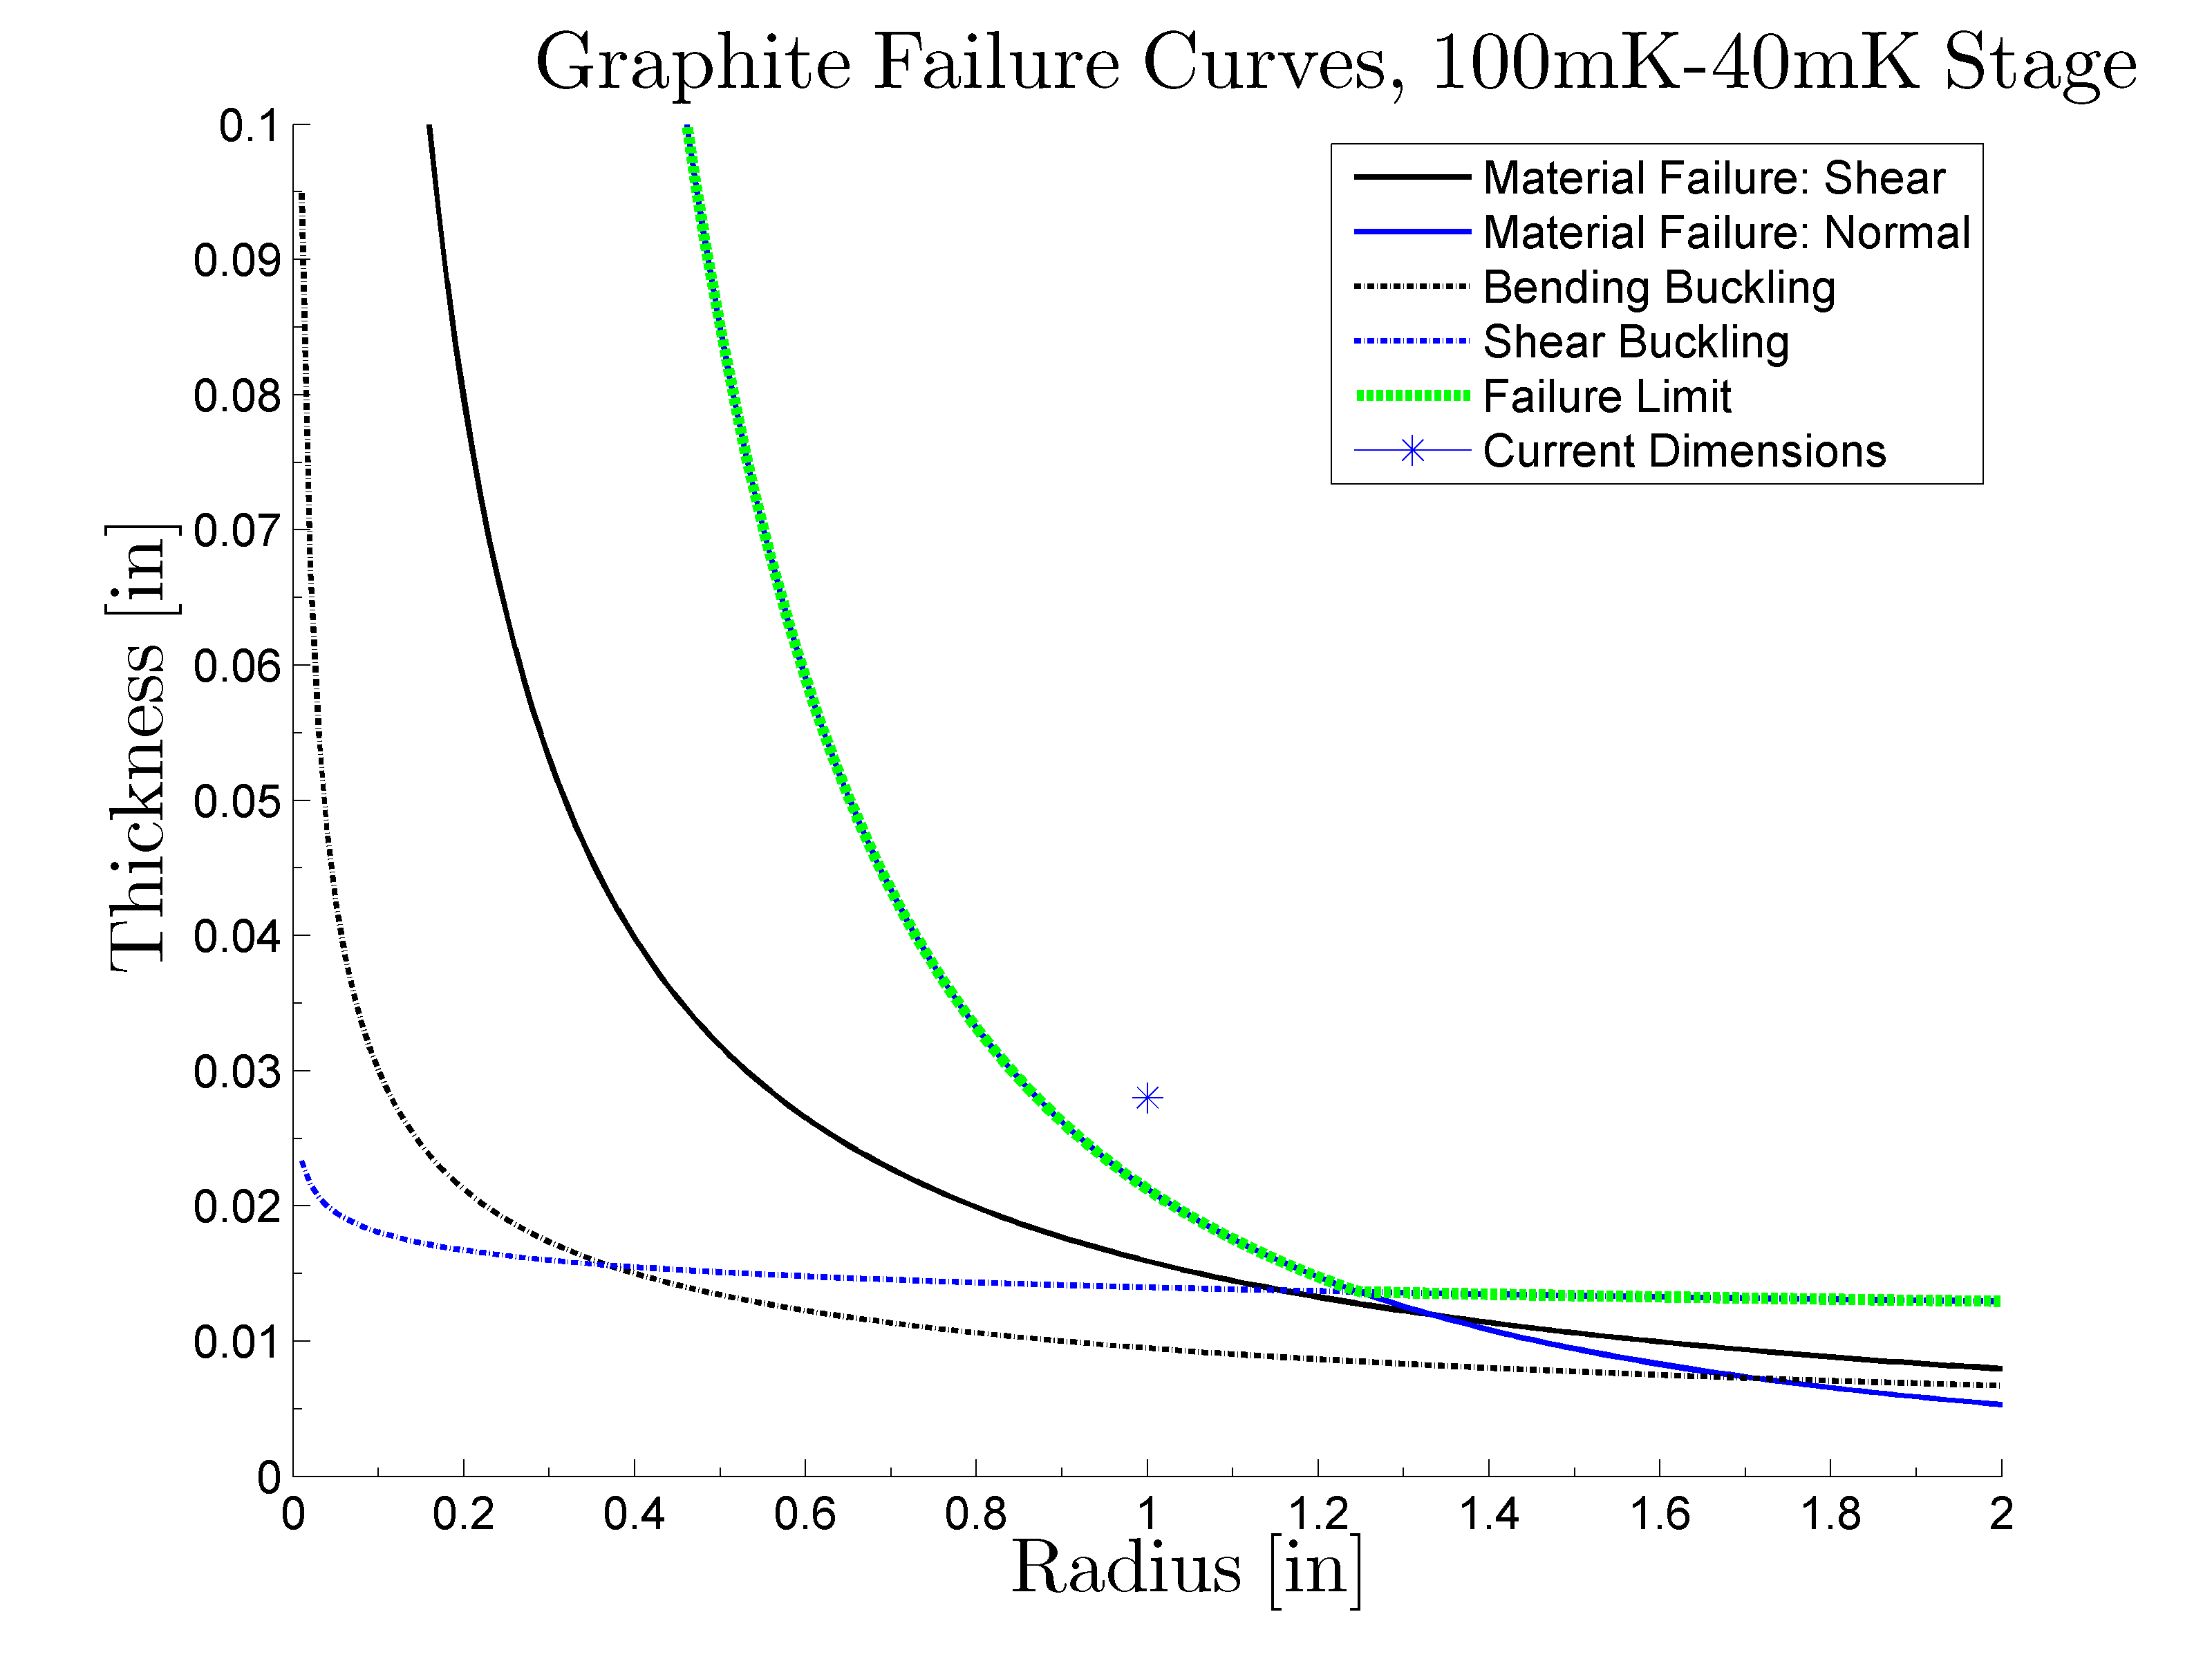
\includegraphics[width=\textwidth]{Graphite_Failure100mK40mK.png}
%\end{minipage}
%\begin{minipage}[t]{.45\textwidth}
%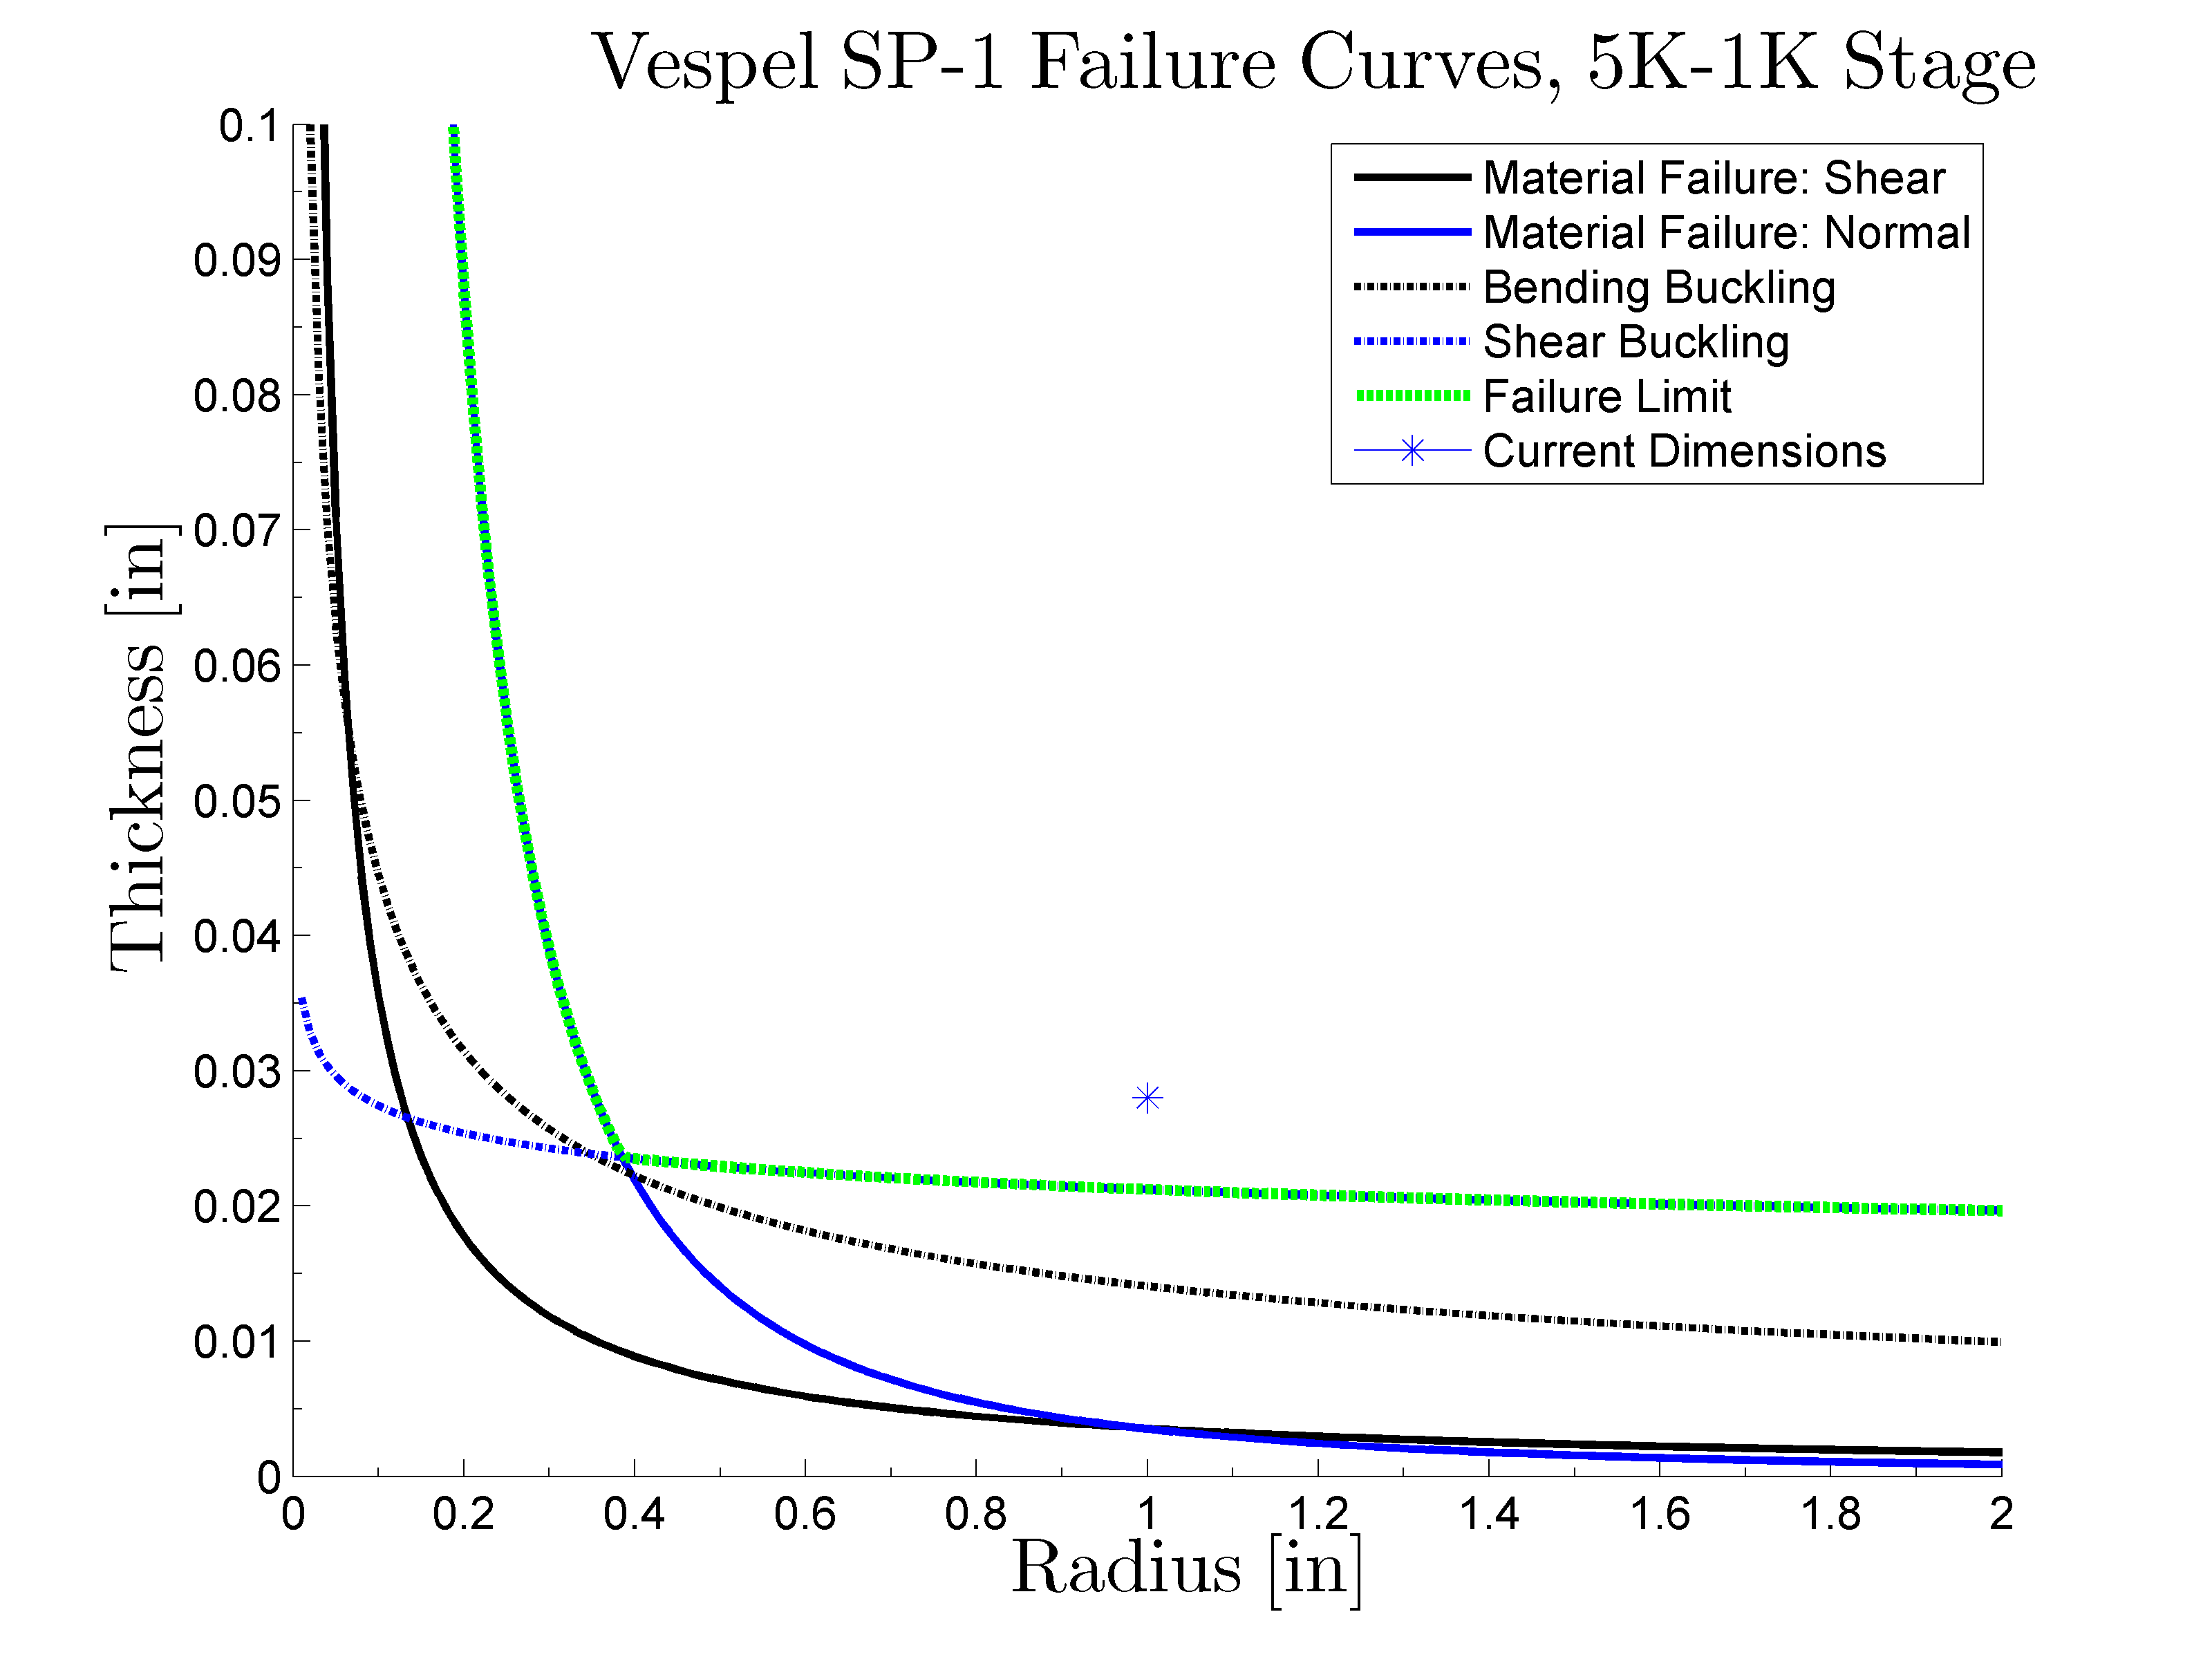
\includegraphics[width=\textwidth]{Vespel_Failure5K1K.png}
%\end{minipage}
%\end{figure}
%\begin{figure}[htb]
%\begin{minipage}[t]{.45\textwidth}
%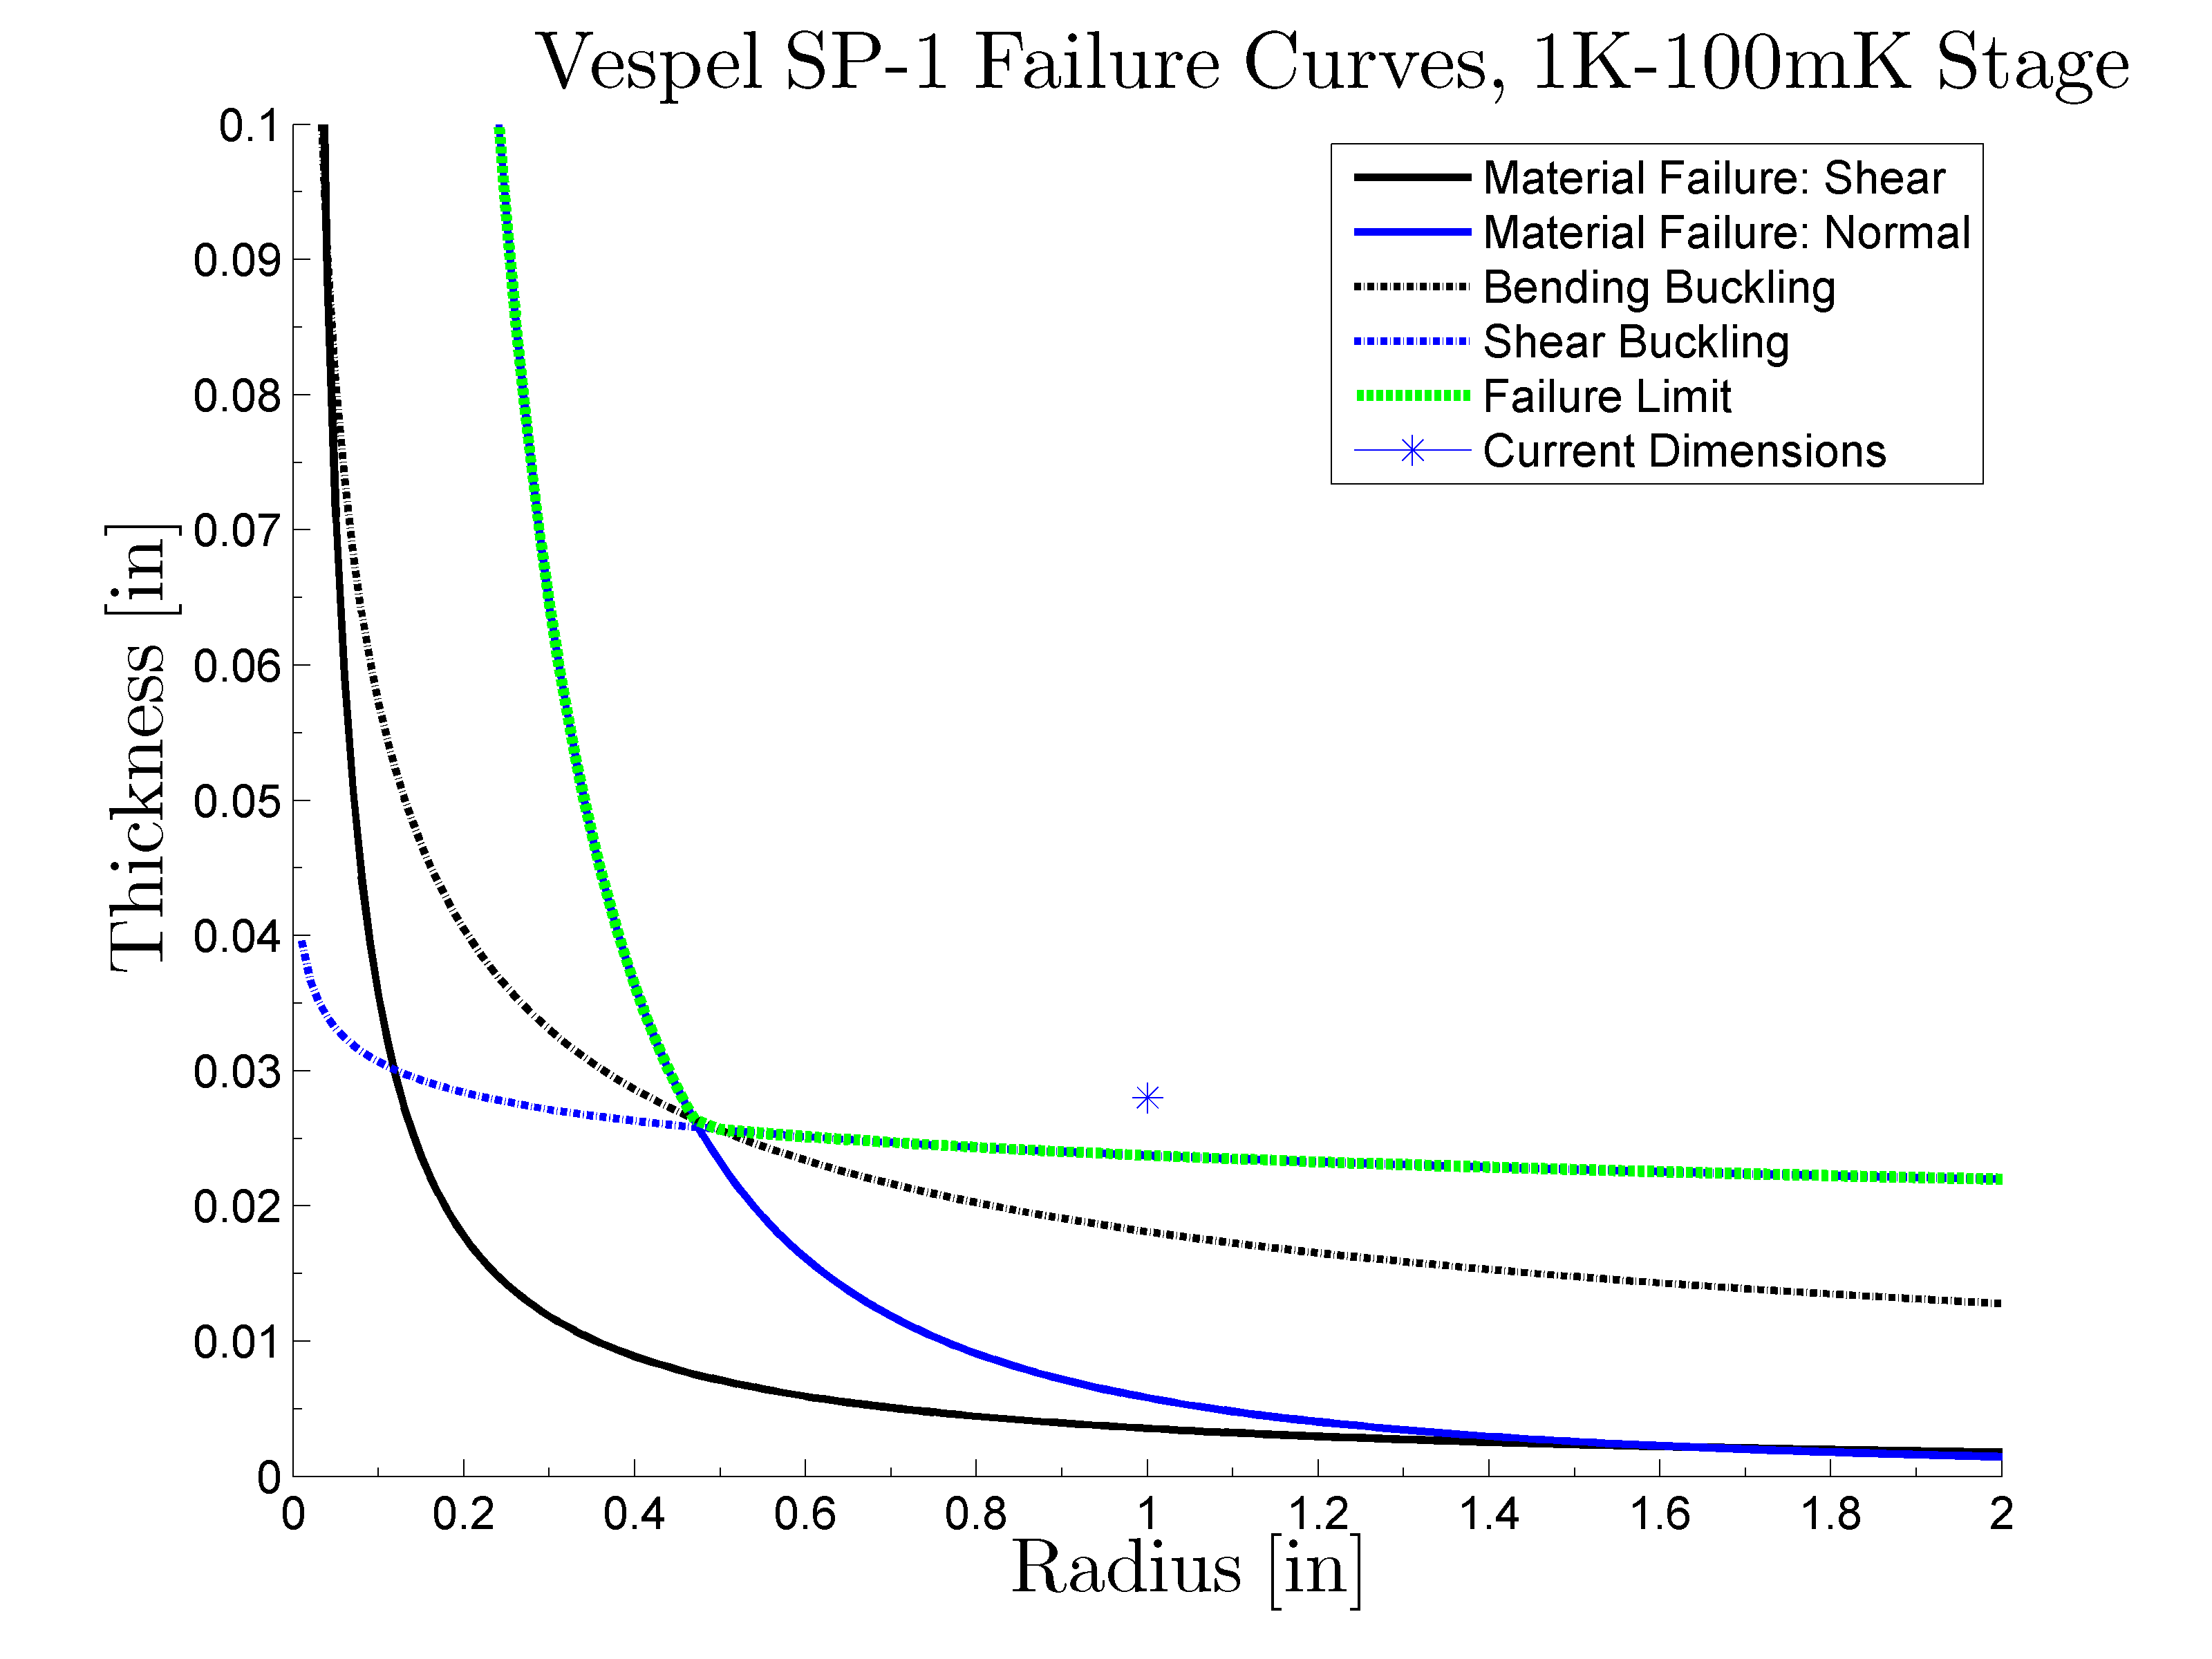
\includegraphics[width=\textwidth]{Vespel_Failure1K100mK.png}
%\end{minipage}
%\begin{minipage}[t]{.45\textwidth}
%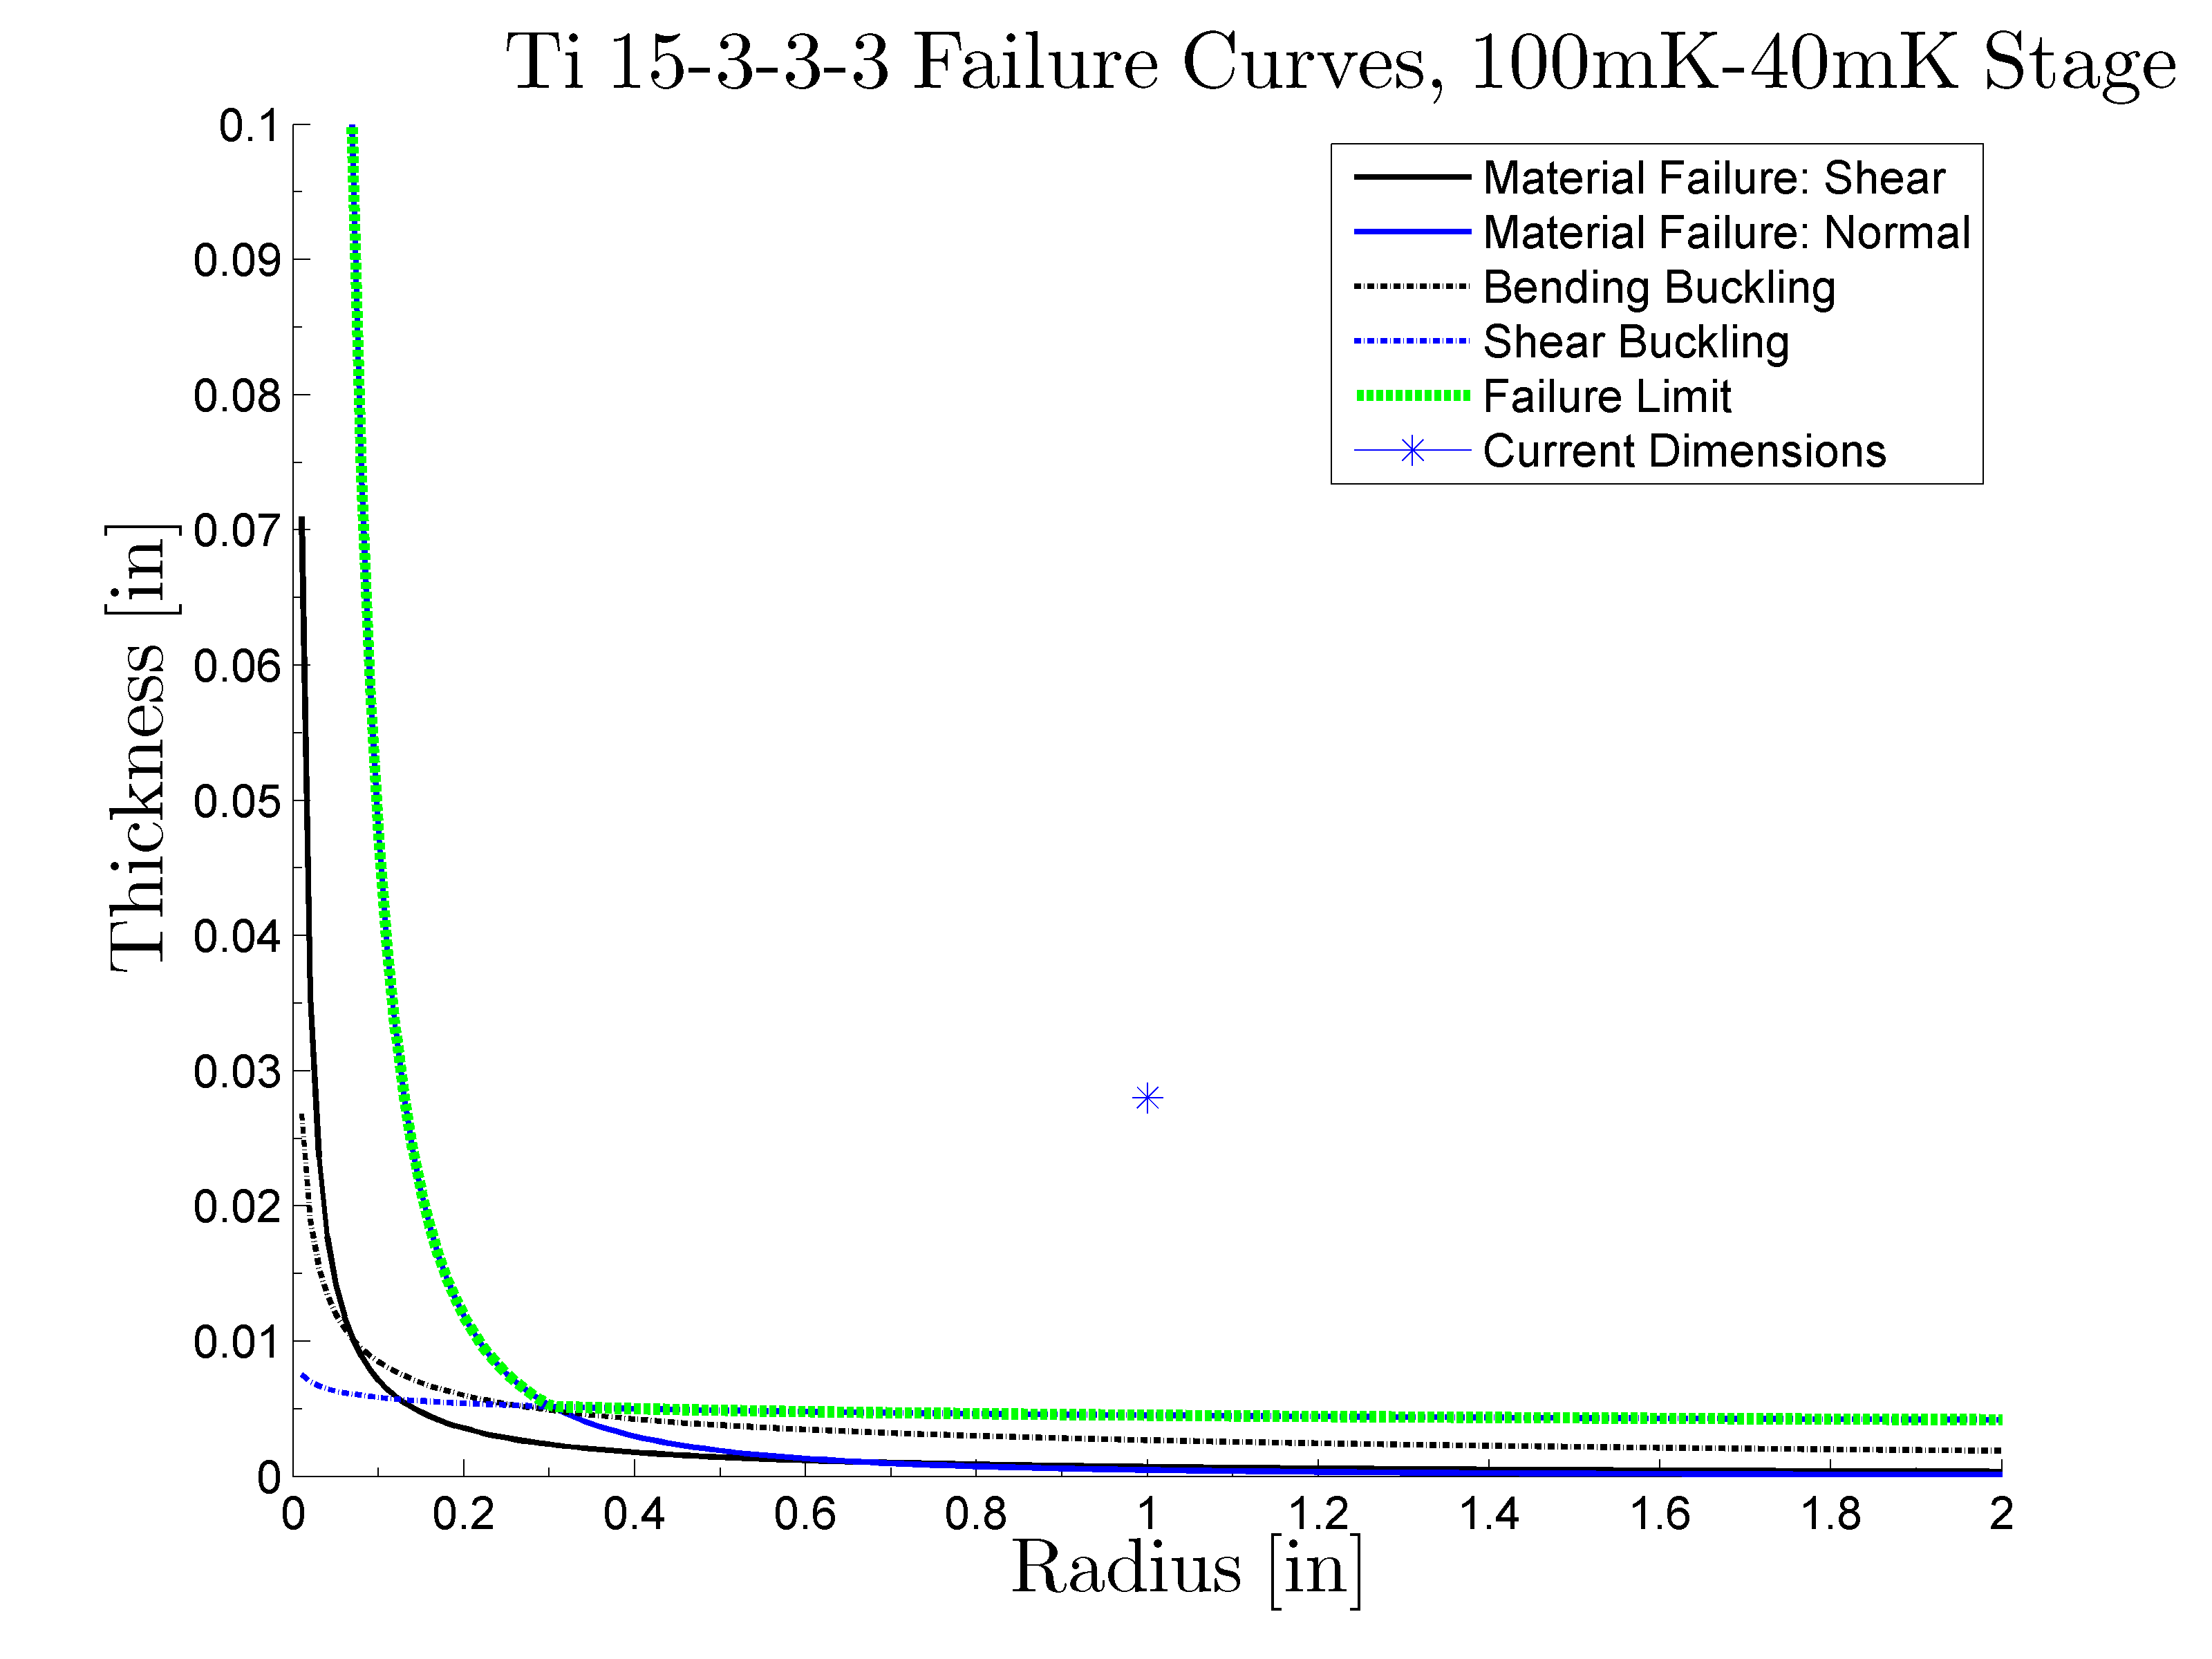
\includegraphics[width=\textwidth]{Ti15333_Failure.png}
%\end{minipage}
%\caption{Theoretical failure curves for different materials for 145lb load. The green dashed line represents minimum (thus optimum) dimensions for a 145lb load. Actual CDMS
%Graphite dimensions are plotted as an '*' for comparison.}
%\end{figure}

The predicted failure curves for CDMS graphite can be seen in the upper-left graph. The predicted dimensions for CDMS Graphite deviate $15-23\%$ from actual values of Radius = 1in, Thickness = 0.028in. The graphite model is still rough, however, as the values of tensile and compressive strength used were those approximated in table 3. These should be verified before further progress is made.

\subsection{Minimizing Radioactivity and Heat Load}

Once the optimal dimension pairs (radius, thickness) are obtained along the failure limit, we can minimize radioactivity and heat load of the candidate materials. Radioactivity is
directly proportional to volume, and thermal power is directly related to cross-sectional area. Holding tube lengths fixed, minimization of radioactivity and heat load is reduced
to the problem of minimizing cross-section. Therefore, radioactivity and heat load will have identical minimization parameters.

The graphs in figure 3 plot radioactivity and thermal power as a function of radius. The thickness of the tube at any radius is implicitly the thickness from the optimal dimension
pairs obtained from the failure limit lines in figure 2.

%\begin{figure}[htb]
%\begin{minipage}[t]{.48\textwidth}
%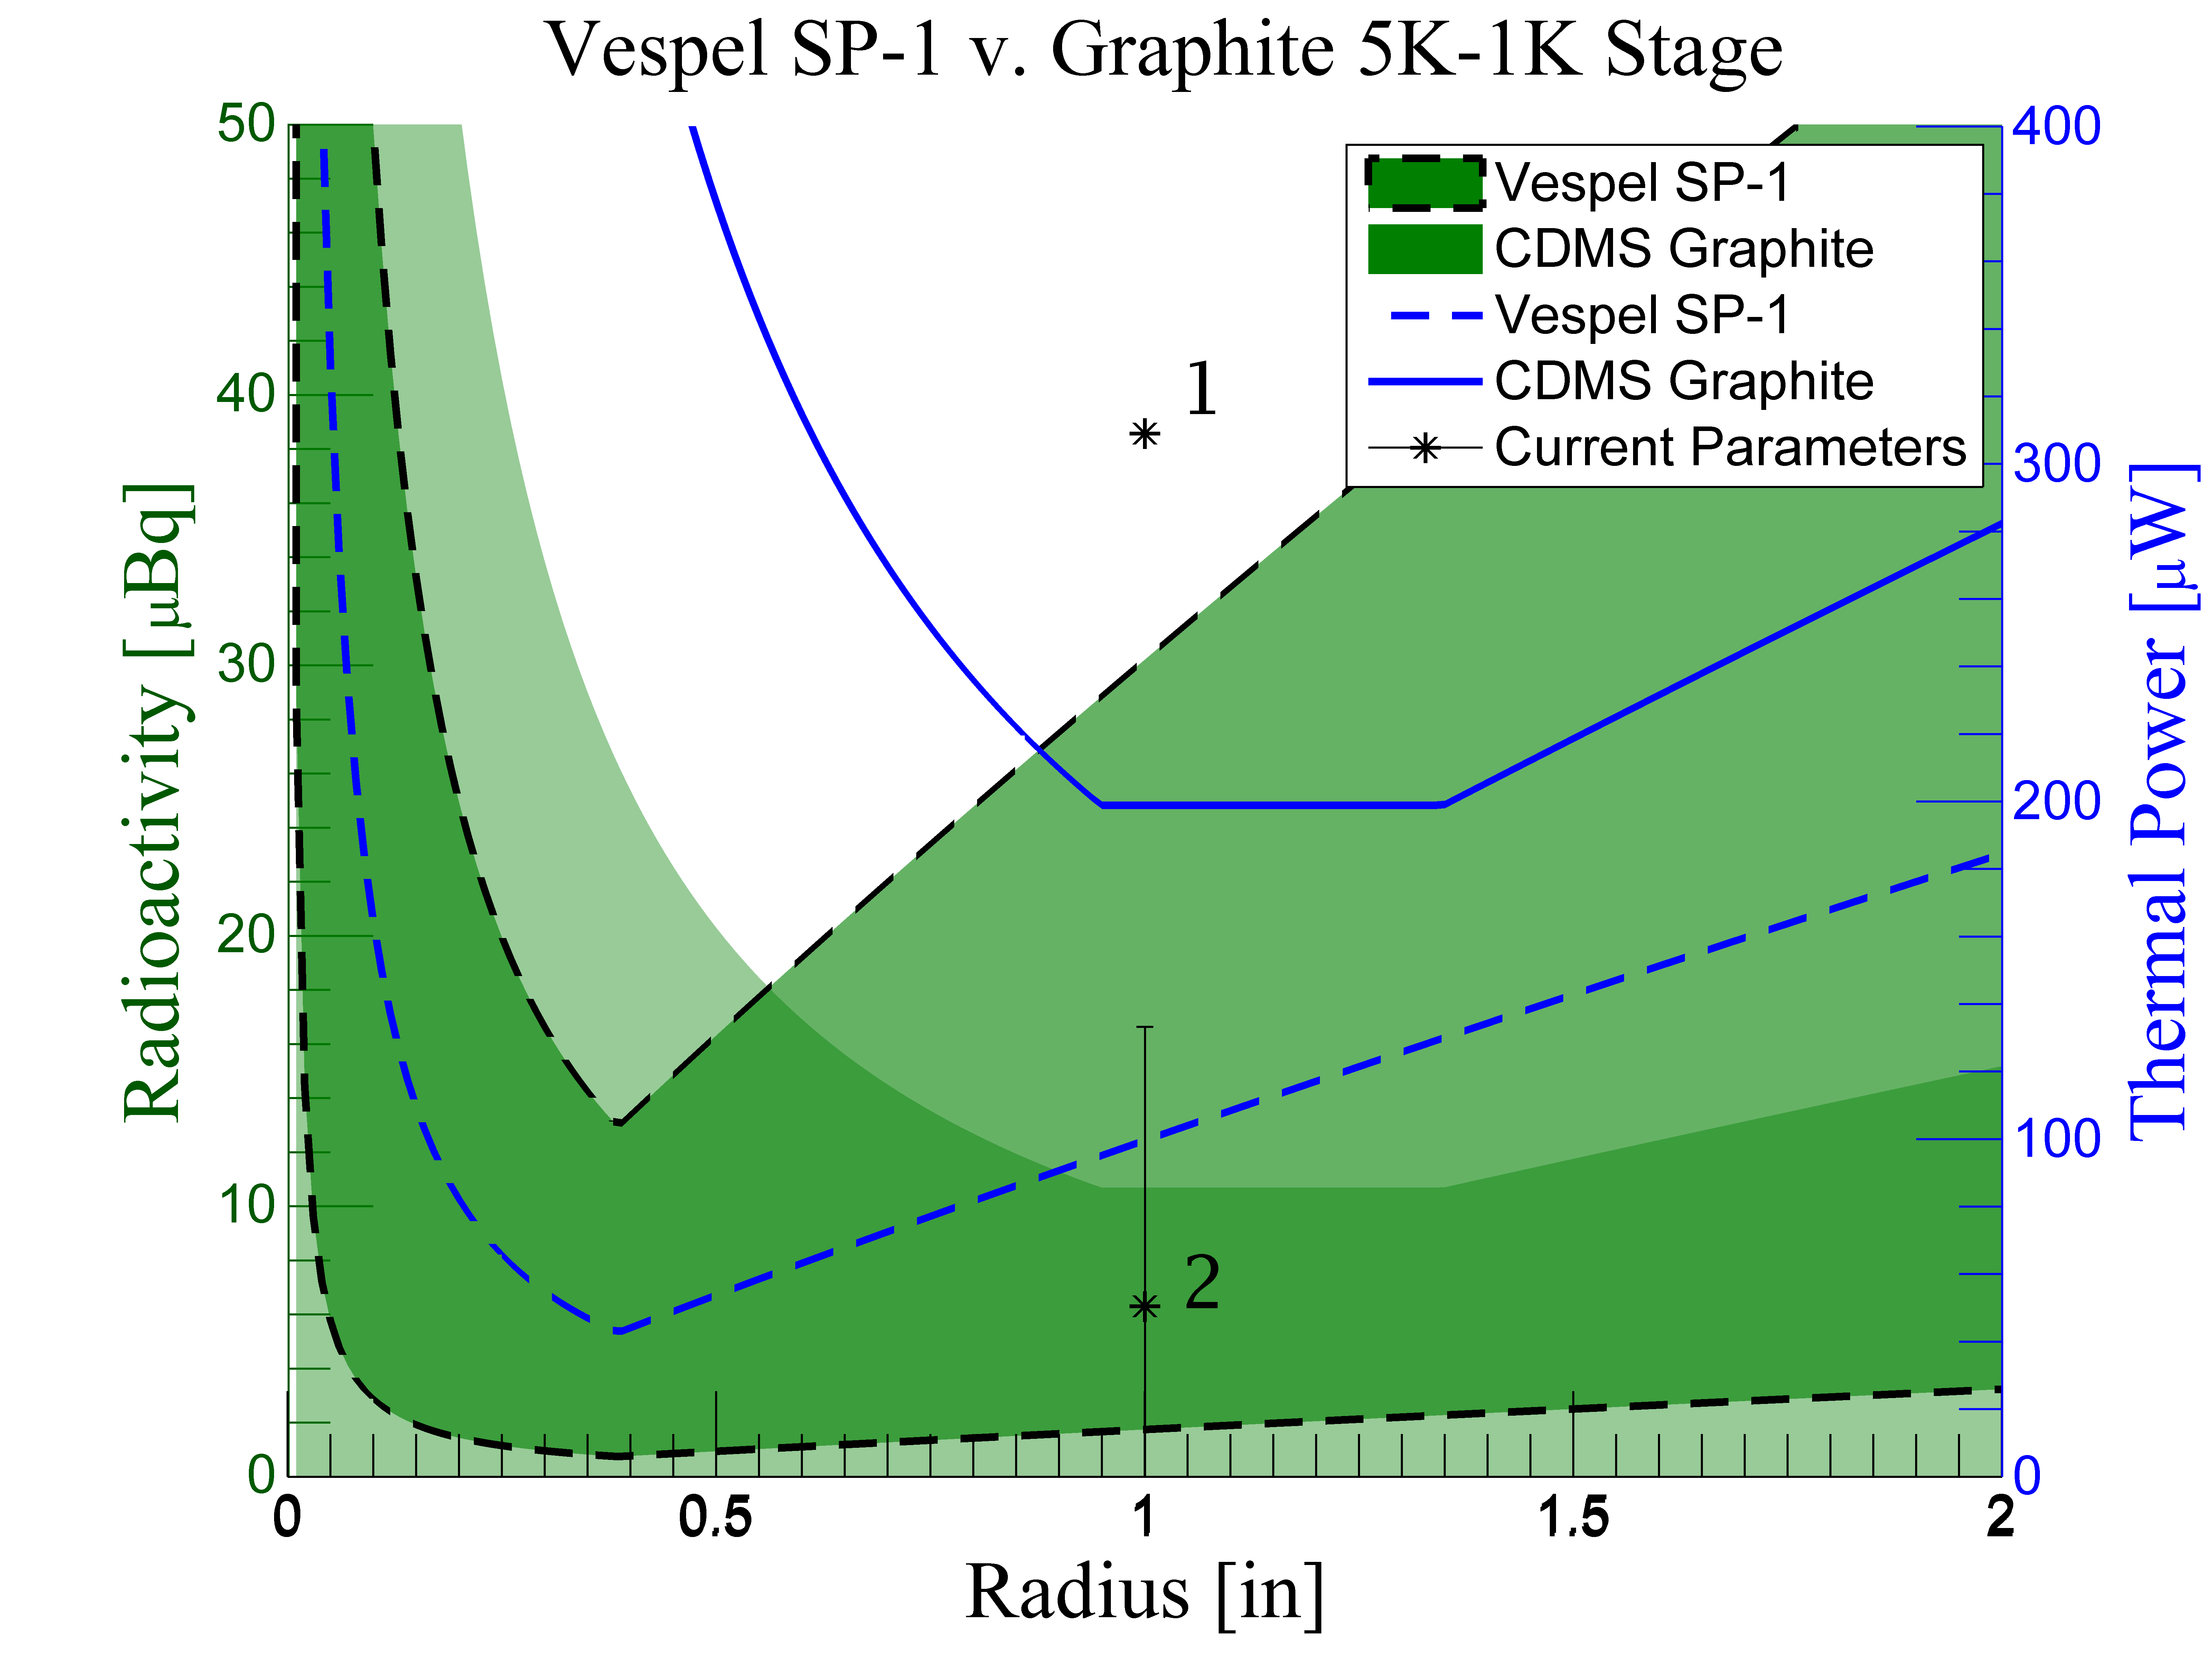
\includegraphics[width=\textwidth]{VSP1_Graphite_5K1K.png}
%\end{minipage}
%\begin{minipage}[t]{.48\textwidth}
%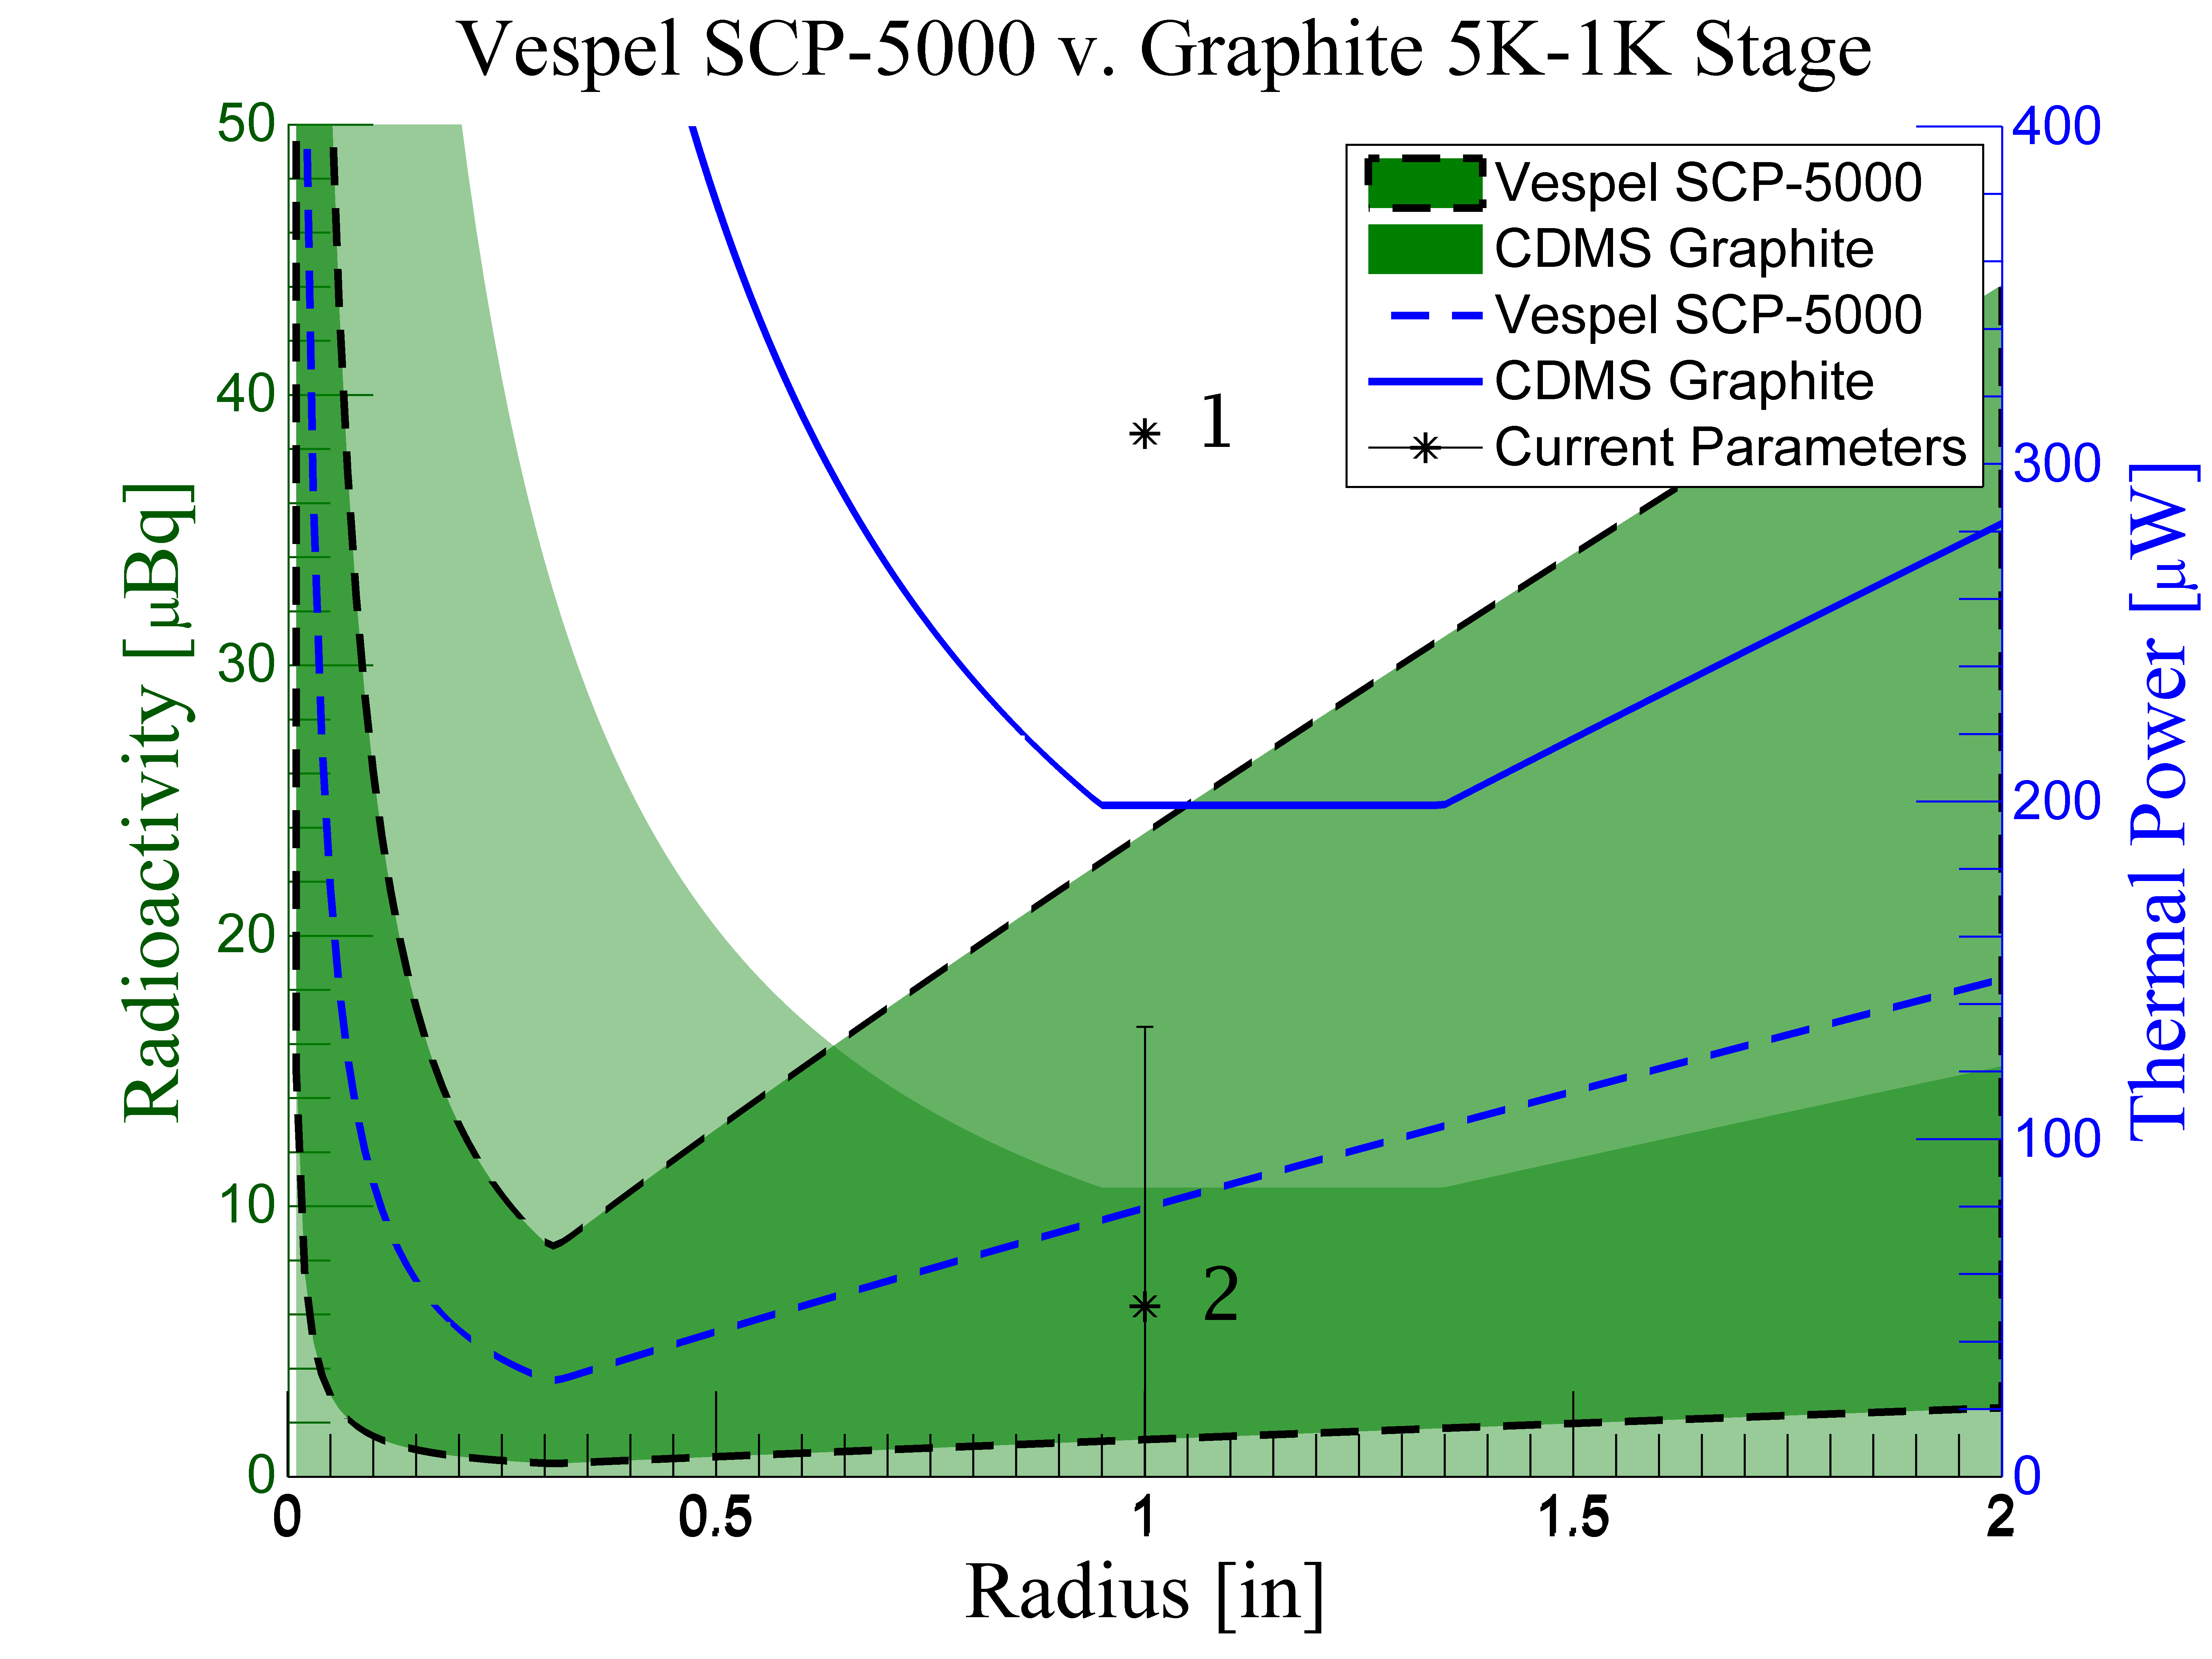
\includegraphics[width=\textwidth]{VSCP5000_Graphite_5K1K.png}
%\end{minipage}
%\end{figure}
%\begin{figure}[htb]
%\begin{minipage}[t]{.48\textwidth}
%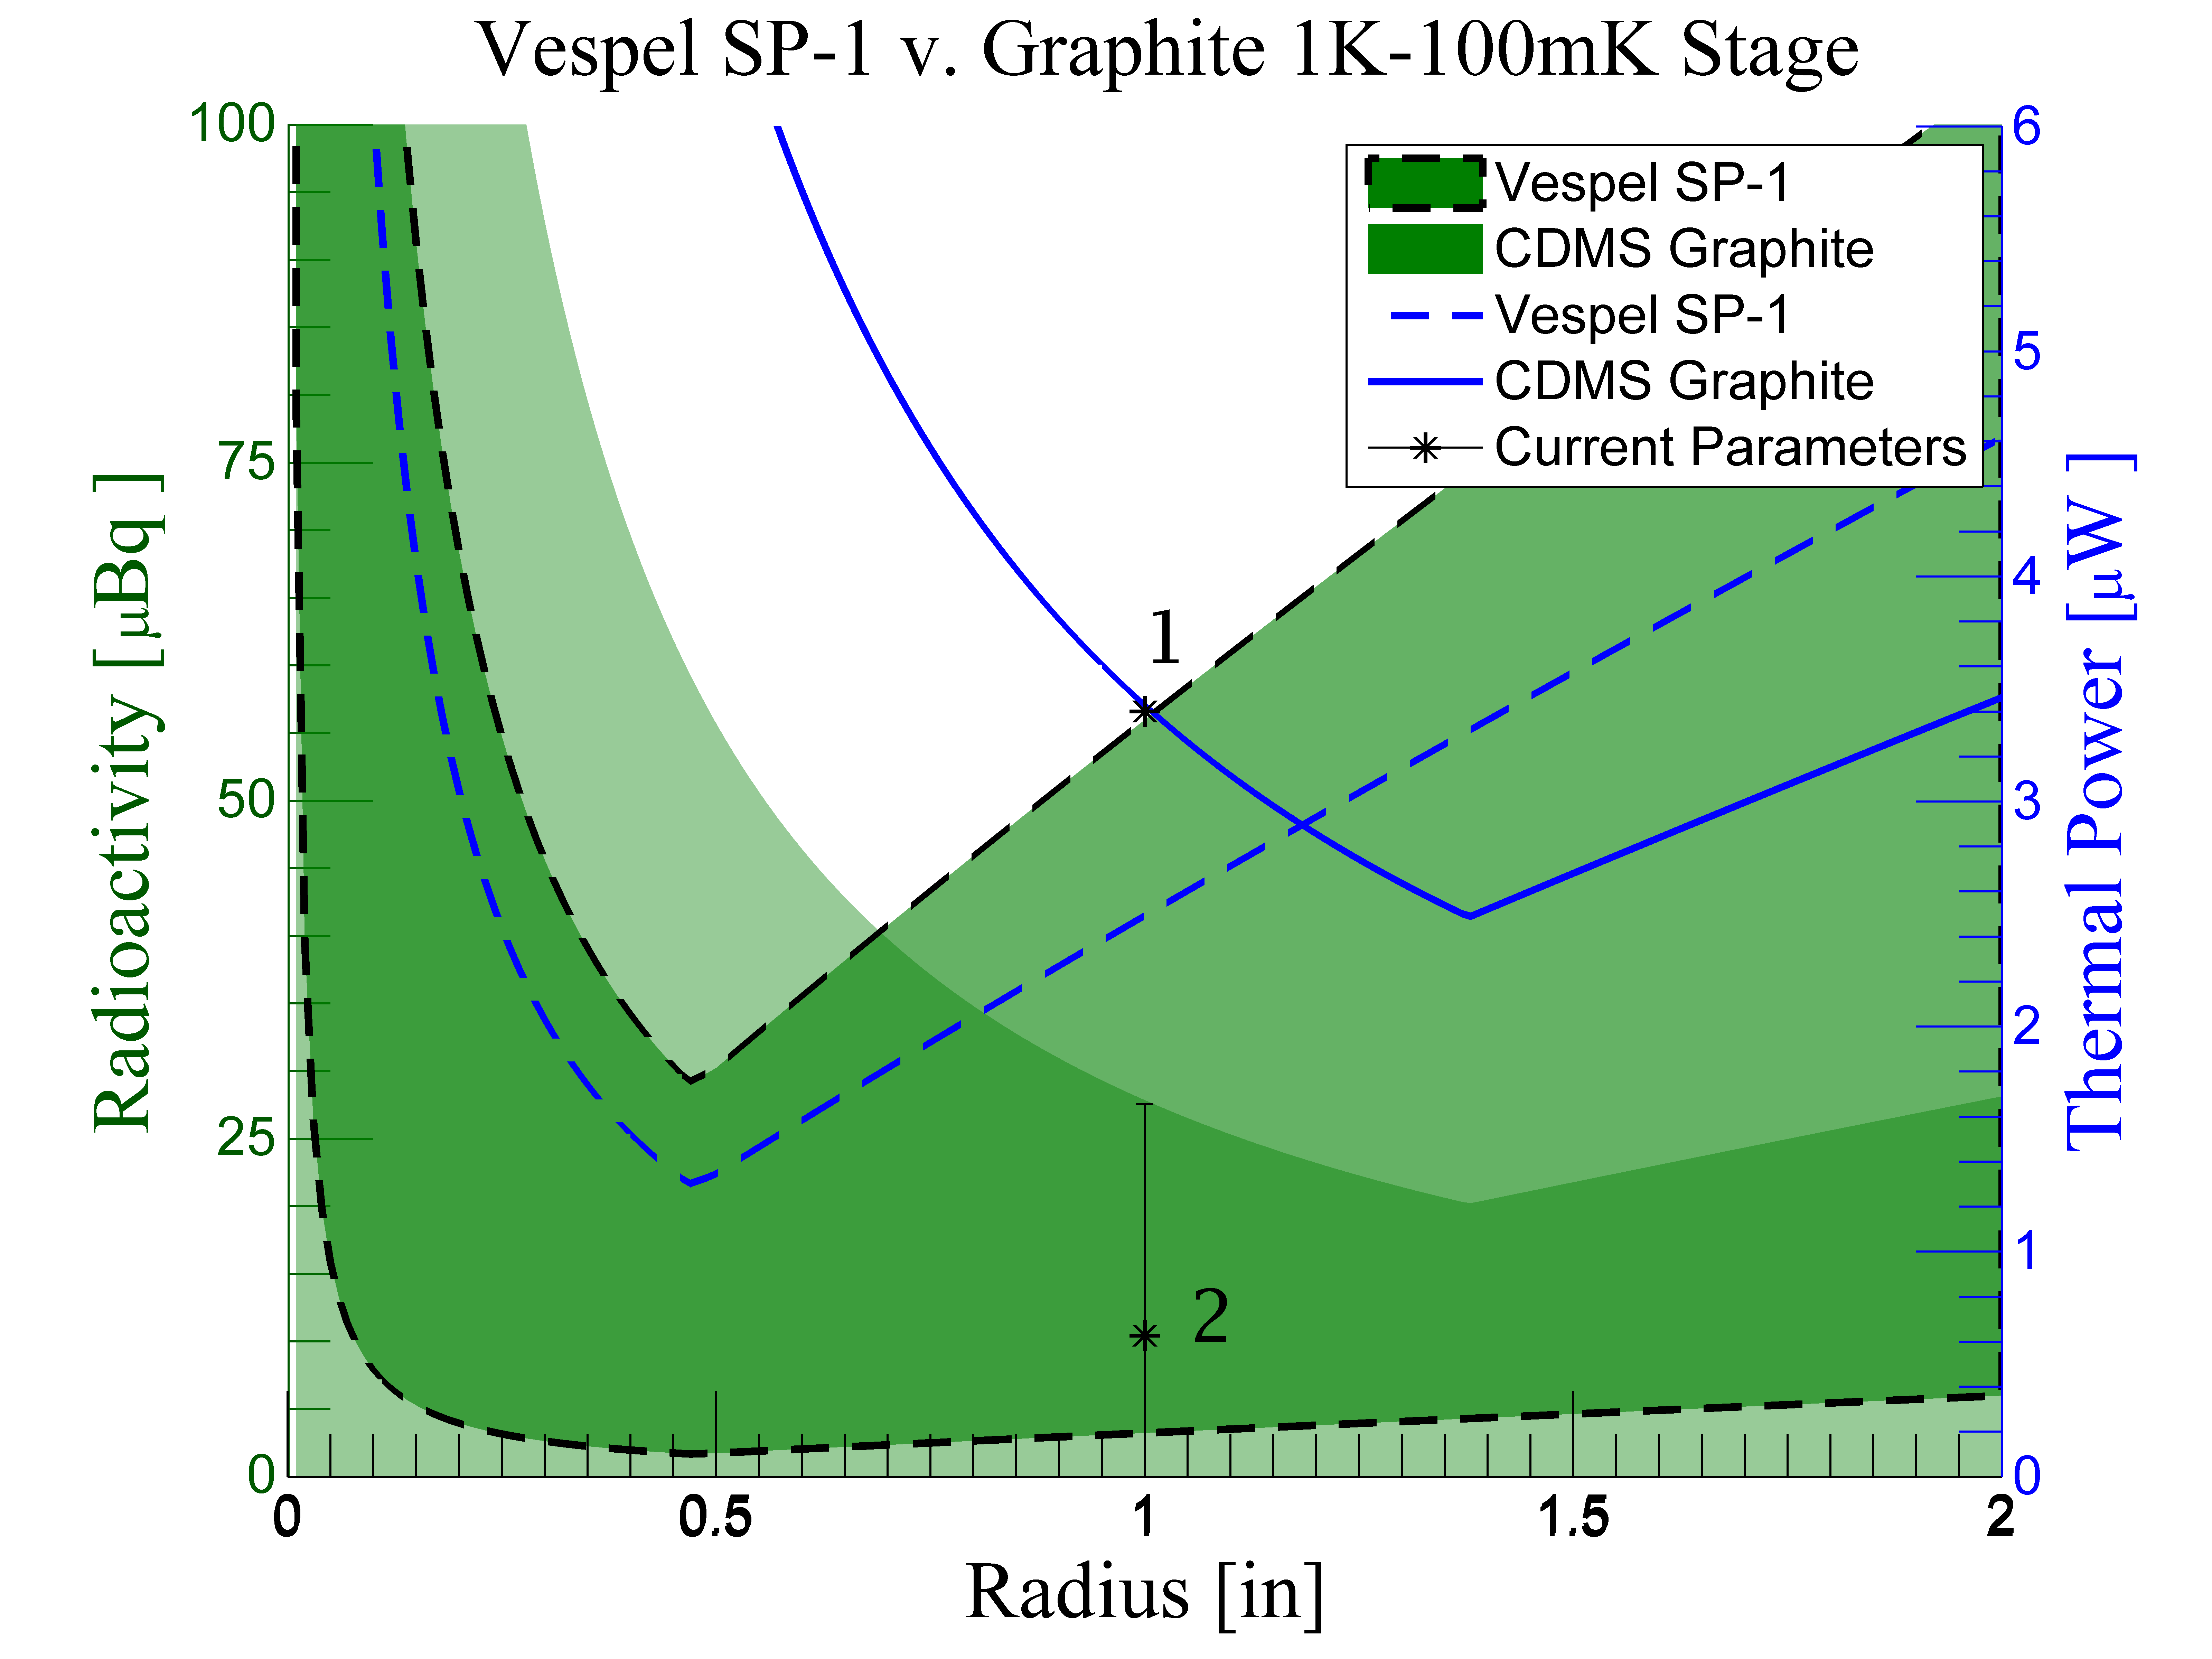
\includegraphics[width=\textwidth]{VSP1_Graphite_1K100mK.png}
%\end{minipage}
%\begin{minipage}[t]{.48\textwidth}
%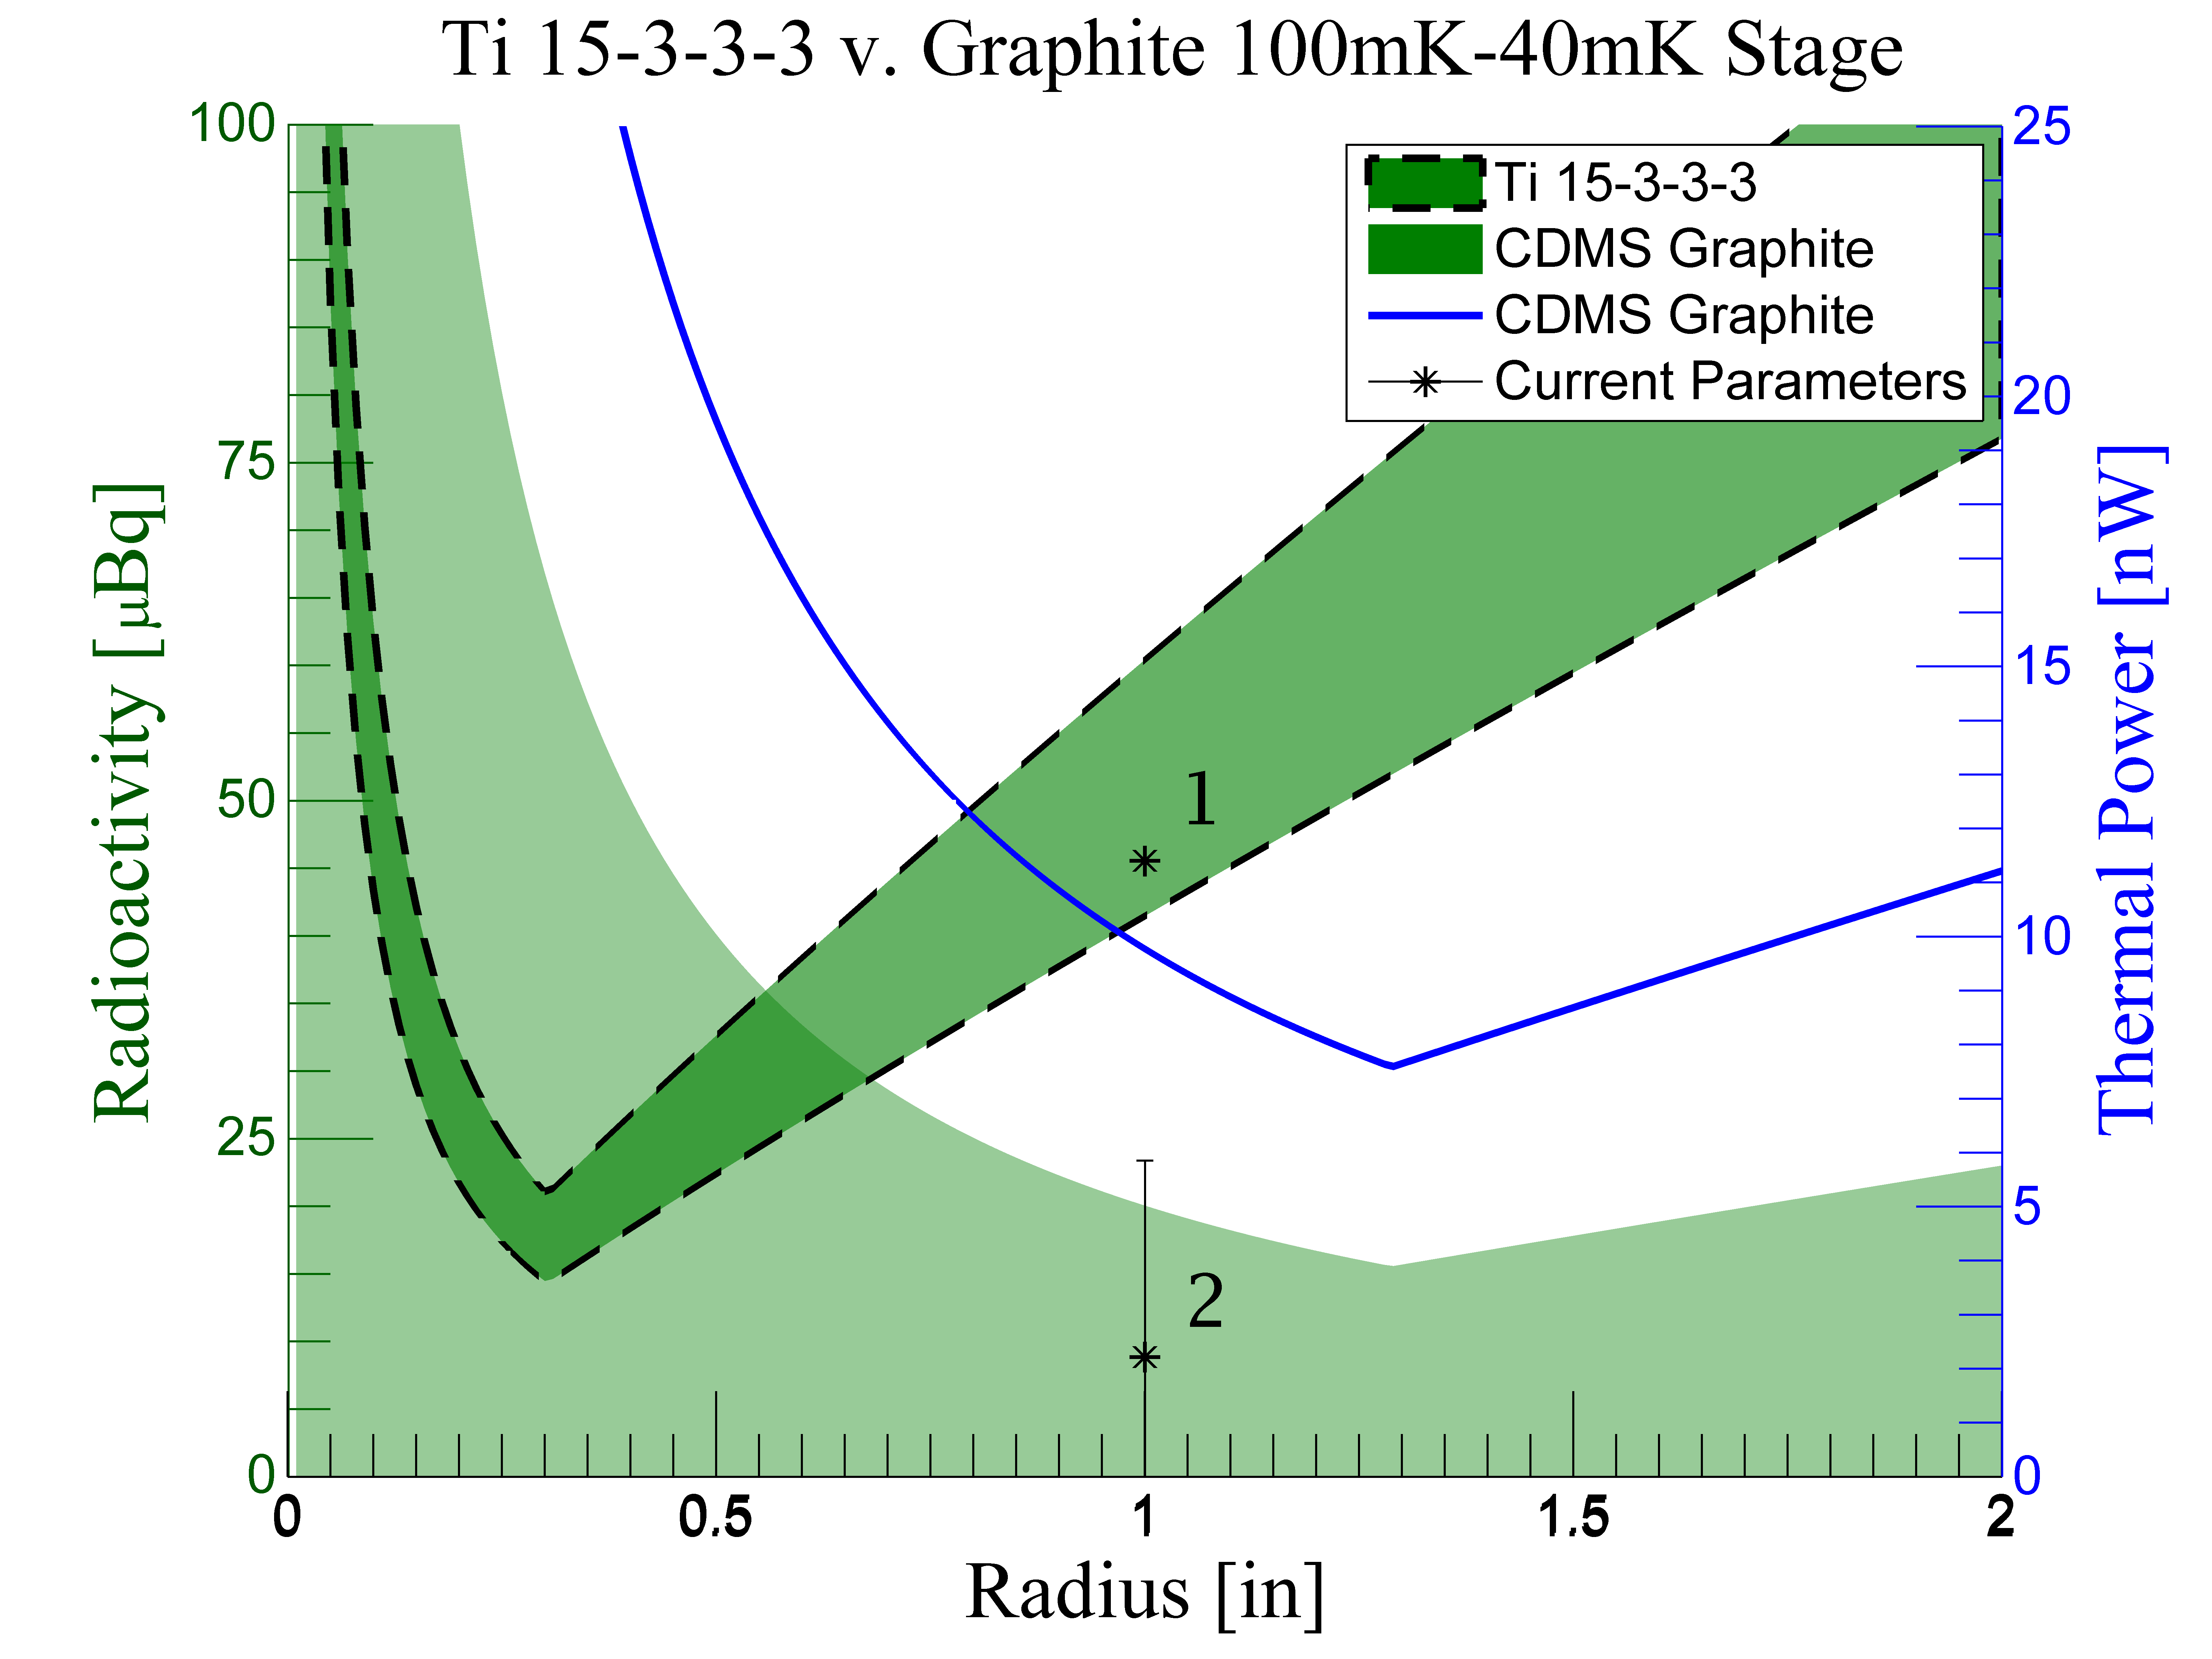
\includegraphics[width=\textwidth]{Ti15333_Graphite_100mK40mK.png}
%\end{minipage}
%\caption{Radioactivity and Thermal Power for varying dimensions. The green shaded regions represent the uncertainty in radioactivity given in table 2. The regions bounded by black
%dashed lines are those of the candidate materials. Point 1 gives current graphite heat load, while point 2 (including error bars) gives current graphite radioactivity.}
%\end{figure}

It is obvious that the candidate materials offer significant improvement over the current UF-4S Graphite. The heat load improvement per stage is examined below. For simplicity,
the values along the optimum lines have been used.

\smallskip

\large{\underline{5K -1K}}

At a radius of 0.4 inches, the power from Vespel SP-1 is 50$\mu$W. This is 1/6 the current heat load. Assuming the same thermal conductivity for Vespel SCP-5000, this number could
be reduced to near 35$\mu$W for more than an 800\% reduction in heat load.

\smallskip

\underline{{\large 1K-100mK}}

Vespel SP-1 could reduce the heat load to 1.3$\mu$W from 3.4$\mu$W, 2.6 times less than the current heat load. Vespel SCP-5000 could offer an additional 30\% improvement over SP-1.

\smallskip

\underline{{\large 100mK-40mK}}

With no data yet in this range for Ti 15-3-3-3 we cannot know the improvement, but at the optimum value, cross-section is reduced by nearly a factor of 20. Given that the thermal
conductivity of Ti 15-3-3-3 is almost certainly lower at this stage than UF-4S Graphite, a significant improvement is expected.

\bigskip

For each stage, the candidate materials not only offer a significant reduction in thermal power, but remain well within acceptable limits for radioactivity.

It should be noted that the optimized values would almost certainly result in a failure load of less than 145lbs. Given the error for the predicted Graphite failure, the actual
would be around 20-30\% lower. Even so, our failure load would still be near 100lbs. If it is decided that this is too low, the material dimensions can easily be increased and
still offer more than a factor of 2 improvement for each stage.

\section{Striplines}
In addition to modifying the tower support tubes, we are examining the feasibility of replacing the NbTi vacuum coaxial cables along tower face with a parallel strip transmission
line. This transmission line must satisfy the new inductance requirements of the SQUID/Detector designs while remaining within acceptable limits for thermal power loading on the
tower stages. Critical current density, resistivity, and critical temperature ($T_{c}$) must also be evaluated for the new line.

Our consideration of a flex cable comes from:
\begin{itemize}
\item Low inductance design capability
\item Precise control over dimensions
\item Reproducibility
\item Strength, and Low Radioactivity (from Kapton substrate)
\end{itemize}

The new SQUID design will reduce the superconducting QET resistance from 0.2$\Omega$ to 0.02$\Omega$. Since the 3dB roll-off frequency corresponds to R/L for our amplifier, when we reduce R by a factor of 10, we must also reduce inductance, L, by a factor of 10 to maintain our bandwidth. The new goal for the inductance of our flex cable is 30nH over a 20 inch length, or $\approx$ 60nH/m. To determine the inductance for our parallel traces we used the following formula used by basic inductance calculators:

$$ L \approx \frac{\mu_{0}\mu_{r}h}{w} \ \ (h > t , w >> h)$$

$\mu_{0}$ = the magnetic constant (4$\pi \cdot 10^{-7}$)\\
$\mu_{r}$ = relative permeability of Kapton (assumed to be 1)\\
t = thickness of trace \\
h = center-to-center separation of traces \\
w = width of the trace \\

Sonnet EM modeling software will be used to provide more detailed inductance modeling as well as to measure electrical cross-talk.

\subsection{NbTi Trace}

We have ordered Nb47Ti(53\% Nb, 47\% Ti by weight) which was rolled by Virginia Fine Metal. The foil is 4" x 10" and 0.002" thick. The same Nb47Ti has already been successfully etched so it can now be made into a preliminary parallel strip transmission line for testing.

\begin{table}[ht]
\centering
\begin{threeparttable}
{\footnotesize\rm\begin{tabular}{l|rrrrrr}
  \multicolumn{7}{l}{{\large Thermal Loading in Tower Stages for Current 8 Pair Design, 6 Face Tower}}\\
\toprule
 {\normalsize Material} & 4.2K-600mK & 600mK-50mK & 50mK - 10mK & 5K-1K\tnote{*} & 1K-100mK\tnote{*} & 100mK-40mK\tnote{*} \\
  &P($\mu$W)&P(nW)&P(nW)&P($\mu$W)& P(nW) & P(nW) \\ \hline\hline
  Ti15333 @ 0.0005" & - & 658.5 & 4.41 & - & 1997 & 15.44 \\
  Ti15333 @ 0.001" & - & 807.4 & 5.03 & - & 2670 & 17.60 \\
  Nb-47Ti @ 0.001" & 108.4 & 879.95 & 5.14  & 170.74 & 2767 & 18.42 \\
  Graphite Tube & 202 & 950 & 2.2 & 309 & 3400 & 11.4 \\
  Current Vacuum Coax's & 0.762 & \multicolumn{2}{r}{3.60} & 1.28 & \multicolumn{2}{r}{16.68} \\
\bottomrule
\end{tabular}
\begin{tablenotes}
   \item[*]{Thermal stability calculations provided to account for non-ideal fridge temperatures}
\end{tablenotes}}
\caption{Calculated power conducted between individual tower stages for 30nH inductance. Graphite numbers based on current support tube lengths: 4.2K-600mK stage - 0.949in; 600mK-50mK
stage - 1.572in; 50mK-10mK stage - 1.334in. Transmission line calculations used inter-stage lengths of: 4.2K-600mK - 0.688in; 600mK-50mK - 0.789in; 50mK-10mK - 0.740in. Vacuum coax
calculations used: 4.2K-600mK - 1.339in; 600mK-10mK - 0.83in. }
\end{threeparttable}
\end{table}

\subsection{Ti 15-3-3-3 Trace}
Ti 15-3-3-3 is another option as a trace material. Its relevant properties are discussed below.
\begin{itemize}
\item Thermal Conductivity: This alloy offers a lower thermal conductivity than NbTi at all stages.
\item Critical Current Density: MUST EXPERIMENTALLY DETERMINE
\item Superconducting Transition Temperature: 3.89K
\item Resistivity: MUST EXPERIMENTALLY DETERMINE
\end{itemize}

Due to it's very low transition temperature, it is not an option at the 4K to 600mK transition. If the SQUIDS are placed at the 600mK stage, Ti 15-3-3-3 is an ideal choice as a trace from 600mK down to the 10mK base.

To roll Ti 15-3-3-3 we have contacted Ulbrich, a company which could provide us with a foil as thin as 0.5 mil. The cost for even 1 mil, however, is \$1010/lb with a minimum of 10 lbs, so it will be expensive. Another possible company is called Arnold Rolled Products. They carry Ti 15-3-3-3 sheet in stock and could roll to 0.5 mil.

\bigskip

\subsection{New 50mK Stage (or 100mK for Non-Ideal) Heatsink}
 The current tower design has an internal heat sink for the 50mK stage. The only external components of this stage on the tower face are two connectors for thermally connecting
the tower support tubes to the fridge. This new transmission line design, while easily adjustable to meet inductance requirements, is much more thermally conductive; therefore,
to implement this new design, I propose adding an additional external component for heatsinking the transmission line to the 50mK fridge stage. The need for an external 50mK
heatsink can be seen in Table 5. We have used a best case transmission line design: 0.5 mil Ti 15-3-3-3 designed for 50nH/20". This is compared to the current NbTi vacuum coax's and graphite tower support tubes. The power shown is per tower with the current 6-sided design.

\bigskip

\begin{table}
\centering
\begin{threeparttable}
\begin{tabular}{l|r}
\multicolumn{2}{c}{Power Loaded to Base (40mK) [nW]}\\\toprule
Ti15333 & 1442 \\\midrule
Current Vacuum Coax's & 16.68\\\midrule
Graphite Tube & 11.4 \\ \bottomrule
\end{tabular}
\end{threeparttable}
\caption{Power load on tower base. For simplicity, only the non-ideal temperature calculations are provided.}
\end{table}

\bigskip
Assuming the internal 50mK stage heatsink can be brought out, we can have  a thermally competitive design for the parallel strip transmission line. Table 4 compares an NbTi line, Ti 15-3-3-3 line, current coax's, and the Graphite tube. NbTi only goes to 1 mil, as it cannot be rolled thinner. Ti 15-3-3-3 is presented in 0.5 mil and 1 mil, as it can be produced in 0.5 mil, but it will be expensive.

\section{Availability}
\subsection{Vespel SP-1/Vespel SCP-5000}

Vespel SP-1 and SCP-5000 are both readily available from DuPont through the certified distributor Curbell Plastics.

As a warning, an employee from Curbell Plastics notified us that another company, Pro Plastics, sells a counterfeit material under the name of Vespel.

\subsection{Carbone UF-4S}

This is the grade currently used in the towers as a support tube. Through recent contact with Mersen (the new owner of Carbone of America) we have found that this grade is still produced and readily available.

\subsection{Ti 15-3-3-3/Ti 21s}

Ti 15-3-3-3 is not available in anything except sheet form in the United States. Chinese companies, however, have Ti 15-3-3-3 available as wire, sheet, and rod. Two possible
companies are YR Titanium and ReTi Metal. Two rods have been ordered from ReTi Metal.

Ti 21s is another metastable-$\beta$ alloy with similar properties to Ti 15-3-3-3. Tests will be conducted to determine its suitability.

\subsection{Stripline Companies}
\subsubsection{Rolling}
\begin{itemize}
\item Hamilton Materials
\item Virginia Fine Metals
\item Arnold Rolled Products
\end{itemize}

\subsubsection{Transmission Line Fabrication}
\begin{itemize}
\item Luxel
\item Tech-Etch
\end{itemize}
\end{multicols}
\newpage

\section{Appendix A: Aluminum as a Candidate Trace Material}

Aluminum is naturally under consideration as a trace material, due to its well known properties and widespread use. Fabrication time for a stripline would be reduced by using Aluminum, as the company fabricating the line, Tech-Etch, has used it as a trace material in the past. A new material, such as Ti15-3-3-3 would require significantly more time to go through the development process. Therefore, it is in our best interest to examine the feasibility of an Aluminum-trace stripline. Considerations for its suitability include its thermal conductivity, coefficient of thermal expansion (CTE), and critical temperature ($T_{c}$).

\subsection{Thermal Conductivity of Al5056}

The Aluminum used by Tech-Etch is 5052-H19, however members of our collaboration were unable to find low temperature thermal conductivity data for this alloy. The thermal conductivity of another alloy, Al5056, was found to be very similar in normal state, so was used a proxy for 5052-H19. The thermal conductivity of Al5056 was determined from \cite{coc} for the range 600mK down to 50mK as,
\begin{equation}
K(T) = 1.9 \cdot 10^{4} T^{2.83} \mu W/cmK
\end{equation}

This thermal conductivity is compared to other phonon stripline candidate materials in Figure 4 below. In the range of interest (600mK - 50mK) we can see that the thermal conductivity of Al5056 is almost two orders of magnitude higher than NbTi and Ti15-3-3-3.

\begin{figure}[h]
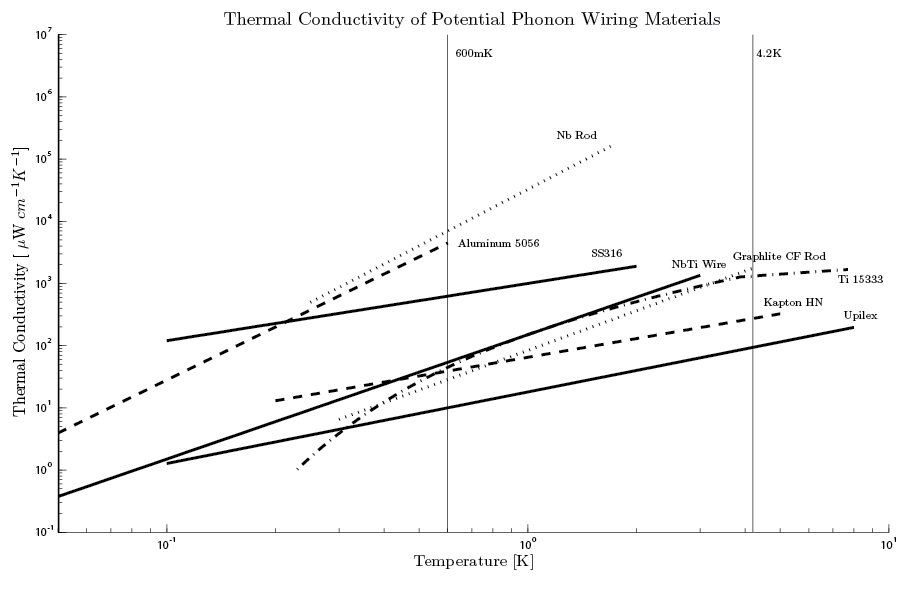
\includegraphics[width = .87\textwidth]{Cable_Therm_Graph.png}
\caption{Thermal conductivities of various stripline candidate materials. The thermal conductivity of Al5056 is nearly two orders of magnitude higher than NbTi or Ti15-3-3-3}
\end{figure}


\subsection{Aluminum Heat Load}

To see if Al will work as a trace material, the thermal power conducted from 600mK to 50mK must be within our thermal budget for the 50mK still of our fridge. The power conducted between a thermal gradient is given by equation 1 in the report. Using a thickness of 1 mil, width of 40 mils, and a trace length of 0.79 inches we can calculate the power for each trace. Assuming 16 traces per detector and 6 detectors per tower, as well as accounting for Kapton heat load, we are able to estimate the total flex cable heat load per tower. The loads for Al5056 are compared with other trace materials in table 7.


\begin{table}
\begin{threeparttable}
\begin{tabular}{l|c|r}
\toprule
Material & Power/Trace [nW] & Total Load per Tower [nW] \\
\midrule
Ti 15-3-3-3 & 0.85 & 684 \\
NbTi & 1.4 & 739 \\
Aluminum & 92 & 9471 \\
\bottomrule
\end{tabular}
\end{threeparttable}
\caption{Estimated heat load for an Aluminum-trace flex cable from 600mK to 50mK as compared with other candidate materials. Assumes 1 mil thick, 40 mils wide, 0.79 inch long traces; 16 traces per detector and 6 detectors per tower.}
\end{table}

The thermal budget for the 50mK end (the still) is $\sim 1 \mu W$. The Al5056 trace heat load is an estimated $9.5 \mu W$ per tower. The heat load for one tower is higher than the thermal budget, though our experiment necessitates the use of multiple towers. Reducing the width of the traces, as well as lengthening the traces could reduce this to perhaps $1\mu W$ (still too high), but inductance constraints would significantly complicate the design.


\section{Thermal Expansion Coefficient of Aluminum}
It is important to match the expansion coefficients of materials which will undergo large temperature changes. In our flex cable, we will be epoxy-ing the Aluminum traces to Kapton polyimide, so the CTE of these two materials should match relatively well. The linear coefficient of thermal expansion presented for Aluminum is 24ppm/K while DuPont states the coefficient for Kapton HN to be 20ppm/K. These values are well matched, so in this regard, Aluminum suites our needs.

\section{Critical Temperature}

The trace material for our striplines must be in a superconducting state for the temperatures at which they are used. The alloy used by Tech-Etch, 5052-H19, has a $T_{c}$ of 775mK. This low $T_{C}$ limits the alloy's use to the 600mK - 50mK span of our flex cable, as it would be in a normal state for most of the 4.2K - 600mK span. The low $T_{c}$ of the alloy is a concern, due to non-ideal temperatures in our fridge. If the temperature drifts upward past the $T_{c}$ of the Aluminum, then the traces will transition to a normal state. Fridge temperatures have been to drift up to as much as 1K, so this is a serious concern for the feasibility of an Aluminum-trace stripline.

\section{Conclusion}

Due to the high thermal conductivity of Aluminum, and the resulting heat load, as well as the low $T_{c}$, our collaboration has decided that it is unsuitable as a trace material.

\newpage

\bibliography{conductivity_rep}


\end{document} 